\documentclass[12pt]{article}

\usepackage[margin=1in,footskip=0.25in]{geometry}
\usepackage{amsmath}
\usepackage{amssymb}
\usepackage{graphicx}
\usepackage{hyperref}
\usepackage{makeidx}

\setcounter{tocdepth}{2}

\hypersetup{
    colorlinks=true,
    linkcolor=blue,       % Color for internal links
    urlcolor=blue         % Color for external URLs
}

% Number equations, figures, and tables within sections
\numberwithin{equation}{section}
\numberwithin{figure}{section}
\numberwithin{table}{section}

\makeindex

\begin{document}

\title{Fluid Mechanics for Ocean Scientists}
\author{Milan Curcic}
\date{}

\maketitle

\tableofcontents

\newpage
\section{Introduction}

\subsection{What will you learn in this course}

The course aims to provide students with a solid understanding of fluid
mechanics fundamentals relevant to ocean physics researchers.
By the end of the course, you will be proficient in applying fluid mechanical
concepts and mathematical tools to solve ocean physics research problems.
The course schedule covers a wide range of topics, starting with a review of
vector calculus and progressing through fluid kinematics, velocity gradients,
strain rates, rotation, and stress. It also includes the conservation of
volume, mass, and momentum, as well as stream functions, velocity potentials,
and Bernoulli's principle. Advanced topics such as vorticity, boundary layers,
turbulence, steady Navier-Stokes equations, flow instabilities, rotating and
stratified flows, and both surface and internal gravity waves are also covered.
The course concludes with a review and discussion session.

\subsection{Reference textbooks}

These lecture notes are based on the following textbooks:

\begin{enumerate}
  \item \textit{Fluid Mechanics}, 6th Ed., by Kundu, Cohen, and Dowling
  \item \textit{Essentials of Atmospheric and Oceanic Dynamics} (EAOD) by Geoffrey Vallis
  \item \textit{Atmospheric and Oceanic Fluid Dynamics} (AOFD) by Geoffrey Vallis.
  This is the longer and more in-depth variant of EAOD.
  Many figures in the notes are adapted from AOFD.
\end{enumerate}

While the notes contain the distilled and required information for you to
succeed in this course, please refer to these textbooks for more detailed
explanations and examples.

\newpage
\section{Review of vector calculus}

In this section we will review the necessary concepts from vector calculus that
we will use in this course.
These include:
scalars, vectors and tensors;
gradient, divergence, and curl;
line, surface, and volume integrals;
and the Gauss and Stokes theorems.

\subsection{Scalars, vectors, and tensors}

In this course we will mainly use three types of quantities to describe fluid
properties: \textit{scalars}, \textit{vectors}, and \textit{tensors}.

\textit{Scalars}\index{Scalar} are completely described by their magnitude.
Examples of scalars are temperature, pressure, or density.
A value of 290 K, for example, completely describes the temperature of a fluid
at some point in space and time.
We will write them in equations using italics, e.g. $T$, $p$, $\rho$.

\textit{Vectors}\index{Vector} have both magnitude and direction.
Examples of vector are velocity, acceleration, or force.
In 3-dimensional Cartesian space with coordinates $(x, y, z)$, for example,
vector $\mathbf{u}(x,y,z)$ can be described by its components

\begin{equation}
  \mathbf{u} =
  \begin{bmatrix}
    u_x \\
    u_y \\
    u_z
  \end{bmatrix}
\end{equation}
where $u_x$, $u_y$, and $u_z$ (each a scalar) are the components of $\mathbf{u}$
in the $x$, $y$, and $z$ directions, respectively.
This is the conventional notation, however, we will often write vectors
inline as $\mathbf{u} = (u_x, u_y, u_z)$.
We will write vectors in equations using boldface, e.g. $\mathbf{u}$,
$\mathbf{a}$, or $\mathbf{F}$.

The magnitude\index{Vector!magnitude}, or norm\index{Vector!norm}, of a 
$\mathbf{u}$ is denoted by $||\mathbf{u}||$, and is calculated as

\begin{equation}
  ||\mathbf{u}|| = \sqrt{u_x^2 + u_y^2 + u_z^2}
\end{equation}

\textit{Tensors}\index{Tensor} have magnitude, direction, and orientation, such as stress or
strain.
They are vectors that act on each respective surface orthogonal to the direction
of the tensor.
In 3-dimensional space, for example, a stress tensor can be described as:

\begin{equation}
  \boldsymbol{\tau} =
  \begin{bmatrix}
    \tau_{xx} & \tau_{xy} & \tau_{xz} \\
    \tau_{yx} & \tau_{yy} & \tau_{yz} \\
    \tau_{zx} & \tau_{zy} & \tau_{zz}
  \end{bmatrix}
\end{equation}
In this notation and index ordering, i.e. $\tau_{ij}$, the first index ($i$)
refers to the direction of the stress component, and the second index ($j$)
refers to the direction of the normal to the surface.
In other words, each row of the tensor contains the three components of a
vector, and each column contains the three surface normals that the stress
component is acting on.
For example, $\tau_{xy}$ is the stress in the x-direction and is acting on the
surface whose normal is in the y-direction (and which lies in the x-z plane).

One special type of tensor is the \textit{identity tensor}\index{Tensor!identity}
$\mathbf{I}$, which is a tensor that maps a vector onto itself.
In Cartesian coordinates, it is given by:

\begin{equation}
  \mathbf{I} =
  \begin{bmatrix}
    1 & 0 & 0 \\
    0 & 1 & 0 \\
    0 & 0 & 1
  \end{bmatrix}
\end{equation}

It may be useful to think of scalars as 0$^{th}$-order tensors, vectors as
1$^{st}$-order tensors, and tensors as 2$^{nd}$-order tensors.\\

\subsection{Unit vectors}

Unit vectors\index{Vector!unit} are vectors with magnitude of 1.
A popular notation for unit vectors in Cartesian coordinates is $\mathbf{i}$,
$\mathbf{j}$, and $\mathbf{k}$, which point in the $x$, $y$, and $z$ directions,
respectively.
So, a vector $\mathbf{u}$ can be written as

\begin{equation}
  \mathbf{u} = u_x \mathbf{i} + u_y \mathbf{j} + u_z \mathbf{k}
\end{equation}

Notice that you can get get the unit vector by dividing any vector by its
magnitude, i.e. $\mathbf{u}/||u||$.

\subsection{Vector operations}

Two vectors can be added, subtracted, or multiplied.
Although vector addition and subtraction are straightforward, vector
multiplication is more interesting.
There are two types of vector multiplication: the \textit{dot product} and the
\textit{cross product}.

\subsubsection{Dot product}

The dot product\index{Product!dot} of two 3-dimensional Cartesian vectors
$\mathbf{a}$ and $\mathbf{b}$ is an element-wise sum of their components
(and thus, a scalar!):

\begin{equation}
  \mathbf{a} \cdot \mathbf{b} =
  \begin{bmatrix}
    a_1 \\
    a_2 \\
    a_3
  \end{bmatrix}
  \cdot
  \begin{bmatrix}
    b_1 \\
    b_2 \\
    b_3
  \end{bmatrix}
  = a_1 b_1 + a_2 b_2 + a_3 b_3
\end{equation}

More generally, the dot product of two n-dimensional vectors $\mathbf{a}$ and
$\mathbf{b}$ is

\begin{equation}
  \mathbf{a} \cdot \mathbf{b} = \sum_{i=1}^{n} a_i b_i = a_1 b_1 + a_2 b_2 + \ldots + a_n b_n
\end{equation}

The dot product is commutative, meaning that
$\mathbf{a} \cdot \mathbf{b} = \mathbf{b} \cdot \mathbf{a}$.

The magnitude of a dot product of two vectors is equal to the product of their
magnitudes and the cosine of the angle $\theta$ between them:

\begin{equation}
  \mathbf{a} \cdot \mathbf{b} = ||\mathbf{a}|| ||\mathbf{b}|| \cos{\theta}
\end{equation}
To visualize this relationship, take one vector and project it onto the other.
This projection is the magnitude of the vector times the cosine of the angle
between them.
Now one vector and the projection of the other onto the first vector are
pointing in the same direction, so their dot product is the product of their
magnitudes.
It can be useful to think of a dot product as collapsing the two vectors into a
single number contains contributions from each of their components.

\subsubsection{Cross product}

The cross product\index{Product!cross} of two vectors $\mathbf{a}$ and
$\mathbf{b}$ is defined as:

\begin{equation}
  \mathbf{a} \times \mathbf{b} =
  det \begin{bmatrix}
    a_x & a_y & a_z \\
    b_x & b_y & b_z \\
    \mathbf{i} & \mathbf{j} & \mathbf{k}
  \end{bmatrix}
\end{equation}
where $det(\mathbf{M})$ means the \textit{determinant of matrix $\mathbf{M}$}.

Using the so-called \textit{rule of Sarrus}, the cross product can be calculated
as:

\begin{equation}
  \mathbf{a} \times \mathbf{b} = (a_y b_z - a_z b_y) \mathbf{i} +
    (a_z b_x - a_x b_z) \mathbf{j} + (a_x b_y - a_y b_x) \mathbf{k}
\end{equation}
or:

\begin{equation}
  \mathbf{a} \times \mathbf{b} =
    \begin{bmatrix}
      a_y b_z - a_z b_y \\
      a_z b_x - a_x b_z \\
      a_x b_y - a_y b_x
    \end{bmatrix}
\end{equation}

The result of a cross product is a vector that is orthogonal to both $\mathbf{a}$
and $\mathbf{b}$.
Its orientation in space is determined by the right-hand rule:
if you point your right thumb in the direction of $\mathbf{a}$ and your index
finger in the direction of $\mathbf{b}$, then your middle finger will point in
the direction of $\mathbf{a} \times \mathbf{b}$.

The magnitude of the cross product is equal to the product of the magnitudes of
the two vectors times the sine of the angle between them:

\begin{equation}
  ||\mathbf{a} \times \mathbf{b}|| = ||\mathbf{a}|| ||\mathbf{b}|| \sin{\theta}
  \label{eq:cross_product_magnitude}
\end{equation}
So, the magnitude of the cross product is largest when the two vectors are
orthogonal.

Unlike the dot product, the cross product is anticommutative, meaning that
$\mathbf{a} \times \mathbf{b} = -\mathbf{b} \times \mathbf{a}$.

In fluid mechanics a cross product will often come up when we are interested in
the rotation of a vector field, such as vorticity.

\subsection{Matrix multiplication}

Occasionally, we will need to multiply a vector by a matrix, or, a matrix by a
matrix.
As a vector is a special case of a matrix in which either the number of rows or
columns is 1, the same rules of matrix multiplication will apply when we
multiply a vector by a matrix or a matrix by a matrix.
These operations are not commutative, meaning that the order of multiplication
matters.

Take two matrices $\mathbf{A}$ and $\mathbf{B}$ such that

\begin{equation}
  \mathbf{A} =
  \begin{bmatrix}
    a_{11} & a_{12} & a_{13} \\
    a_{21} & a_{22} & a_{23} \\
    a_{31} & a_{32} & a_{33}
  \end{bmatrix}
\end{equation}
and:

\begin{equation}
  \mathbf{B} =
  \begin{bmatrix}
    b_{11} & b_{12} & b_{13} \\
    b_{21} & b_{22} & b_{23} \\
    b_{31} & b_{32} & b_{33}
  \end{bmatrix}
\end{equation}

The result of their multiplication is a matrix $\mathbf{C}$ given by:

\begin{equation}
  \mathbf{C} = \mathbf{A} \mathbf{B} =
  \begin{bmatrix}
    a_{11} b_{11} + a_{12} b_{21} + a_{13} b_{31} &
    a_{11} b_{12} + a_{12} b_{22} + a_{13} b_{32} &
    a_{11} b_{13} + a_{12} b_{23} + a_{13} b_{33} \\
    a_{21} b_{11} + a_{22} b_{21} + a_{23} b_{31} &
    a_{21} b_{12} + a_{22} b_{22} + a_{23} b_{32} &
    a_{21} b_{13} + a_{22} b_{23} + a_{23} b_{33} \\
    a_{31} b_{11} + a_{32} b_{21} + a_{33} b_{31} &
    a_{31} b_{12} + a_{32} b_{22} + a_{33} b_{32} &
    a_{31} b_{13} + a_{32} b_{23} + a_{33} b_{33}
  \end{bmatrix}
\end{equation}

That is, the entry $c_{ij}$ of the product is obtained by multiplying
term-by-term the entries of the $i$-th row of $\mathbf{A}$ and the $j$-th column
of $\mathbf{B}$, and summing these products.
In other words, $c_{ij}$ is the dot product of the $i$-th row of $\mathbf{A}$
and the $j$-th column of $\mathbf{B}$.

\subsection{Total and partial derivatives}

We will denote total\index{Derivative!total} and partial\index{Derivative!partial}
derivative operators (for example, in time $t$)
as $\frac{d}{dt}$ and $\frac{\partial}{\partial t}$.
Scalars, vectors, and tensors alike can be differentiated with respect to any
variable.
A derivative of a vector is simply a vector of derivatives of its components:

\begin{equation}
  \frac{d\mathbf{u}}{dt}
    = (\frac{d u_x}{d t}, \frac{d u_y}{d t}, \frac{d u_z}{d t})
    = \frac{du_x}{dt} \mathbf{i} + \frac{du_y}{dt} \mathbf{j} + \frac{du_z}{dt} \mathbf{k}
    = \begin{bmatrix}
        \frac{du_x}{dt} \\
        \frac{du_y}{dt} \\
        \frac{du_z}{dt}
      \end{bmatrix}
\end{equation}

\begin{equation}
  \frac{\partial \mathbf{u}}{\partial t}
    = (\frac{\partial u_x}{\partial t}, \frac{\partial u_y}{\partial t}, \frac{\partial u_z}{\partial t})
    = \frac{\partial u_x}{\partial t} \mathbf{i} + \frac{\partial u_y}{\partial t} \mathbf{j} + \frac{\partial u_z}{\partial t} \mathbf{k}
    = \begin{bmatrix}
        \frac{\partial u_x}{\partial t} \\
        \frac{\partial u_y}{\partial t} \\
        \frac{\partial u_z}{\partial t}
      \end{bmatrix}
\end{equation}
and likewise for tensors.\\

\subsection{Gradient, divergence, and curl}

Now, we introduce another new operator that builds on top of previous
concepts to describe how scalar and vector fields change in space.
This operator is called \textit{del}\index{Del} and is denoted by the symbol
$\nabla$\index{Nabla} (pronounced "nabla"):

\begin{equation}
  \label{eq:nabla}
  \nabla = \frac{\partial}{\partial x} \mathbf{i} +
    \frac{\partial}{\partial y} \mathbf{j} +
    \frac{\partial}{\partial z} \mathbf{k}
\end{equation}

A good way to think about $\nabla$ is as of a \textit{differential operator},
which itself is a 3-dimensional vector that can operate on scalars or vectors.
Specifically:

\begin{itemize}
  \item $\nabla p$ is as vector that is a gradient of a scalar field $p$;
  it quantifies how $p$ changes in space.
  \item $\nabla \cdot \mathbf{u}$ is a scalar that is the divergence of a vector
  field $\mathbf{u}$; it quantifies how $\mathbf{u}$ flows out of a point.
  \item $\nabla \times \mathbf{u}$ is a vector that is the curl of a vector field
  $\mathbf{u}$; it quantifies how $\mathbf{u}$ rotates around a point.
\end{itemize}

Although, strictly speaking, one is a symbol and the other is an operator,
$\nabla$ ("nabla") and "del" are often used interchangeably.

\subsubsection{Gradient}

The gradient\index{Gradient} of a scalar field $T$ is a vector field that points in the
direction of the greatest rate of increase of $T$.
It is denoted by $\nabla T$ and is defined as

\begin{equation}
  \nabla T = \frac{\partial T}{\partial x} \mathbf{i} +
    \frac{\partial T}{\partial y} \mathbf{j} +
    \frac{\partial T}{\partial z} \mathbf{k}
\end{equation}

Gradient of a scalar field is a vector that points in the direction of the
steepest increase of that field, and its magnitude is the rate of that increase.
For example, imagine hiking up a hill; the gradient of the terrain is a vector
that is pointing toward the steepest incline, and its magnitude is the slope
of that incline.

\subsubsection{Divergence}

The divergence\index{Divergence} of a vector field $\mathbf{u}$ is a scalar field that describes
the rate at which the vector field flows out of a point.
It is denoted by $\nabla \cdot \mathbf{u}$ and is defined as

\begin{equation}
  \label{eq:divergence}
  \nabla \cdot \mathbf{u} = \frac{\partial u_x}{\partial x} +
    \frac{\partial u_y}{\partial y} + \frac{\partial u_z}{\partial z}
\end{equation}

Divergence of a vector field is a scalar that describes how much the vector
field is expanding or contracting at a point.
When divergence is negative, it is commonly referred to as convergence.

\subsubsection{Curl}

The curl\index{Curl} of a vector field $\mathbf{u}$ is a vector field that describes the
rotation of the vector field.
It is denoted by $\nabla \times \mathbf{u}$ and is defined as

\begin{equation}
  \nabla \times \mathbf{u} = \left( \frac{\partial u_z}{\partial y} -
    \frac{\partial u_y}{\partial z} \right) \mathbf{i} +
    \left( \frac{\partial u_x}{\partial z} -
    \frac{\partial u_z}{\partial x} \right) \mathbf{j} +
    \left( \frac{\partial u_y}{\partial x} -
    \frac{\partial u_x}{\partial y} \right) \mathbf{k}
\end{equation}

Curl of a vector field is another vector that is orthogonal to the original
vector field and quantifies how much the vector field is rotating around a
point.
When curl is zero, the vector field is said to be \textit{irrotational}.

\subsection{Gauss and Stokes theorems}

The most useful in our work will be variants of the
\textit{Gauss and Stokes theorems}.
The Gauss theorem relates a volume integral of a divergence of a vector field
to a surface integral of that vector field.
The Stokes theorem relates a surface integral of the curl of a vector field to
a line integral of that vector field.
Here, these are merely stated for reference.
We will explore their meaning and application in more detail as we use them
to derive the fundamental equations for fluid flows.

\subsubsection{Gauss theorem}

The Gauss theorem\index{Theorem!Gauss} states that the volume integral of the
divergence of a vector field $\mathbf{u}$ over a volume $V$ is equal to the
surface integral of $\mathbf{u}$ over the surface $A$ that encloses $V$:

\begin{equation}
  \label{eq:divergence_theorem}
  \int_V \nabla \cdot \mathbf{u} dV = \oint_A \mathbf{u} \cdot d\mathbf{A}
\end{equation}

This form of Gauss's theorem is also known as the
\textit{divergence theorem}\index{Theorem!divergence}.
It will come in handy when we derive the conservation of mass (continuity)
equation.

\subsubsection{Stokes theorem}

The Stokes theorem\index{Theorem!Stokes} states that the surface integral of the curl of a
vector field $\mathbf{u}$ over a surface $A$ is equal to the line integral of
$\mathbf{u}$ over the boundary of $A$:

\begin{equation}
  \int_A (\nabla \times \mathbf{u}) \cdot d\mathbf{A} = \oint_{\partial A} \mathbf{u} \cdot d\mathbf{l}
\end{equation}

\subsection{Summary}

In this chapter, we reviewed:

\begin{itemize}
  \item Scalars, vectors, and tensors;
  \item Vector algebra: dot product ($\mathbf{a} \cdot \mathbf{b}$) and cross
  product ($\mathbf{a} \times \mathbf{b}$);
  \item Derivatives: total ($\frac{d}{dt}$) and partial ($\frac{\partial}{\partial t}$);
  \item Gradient, divergence ($\nabla \cdot \mathbf{u}$), and curl ($\nabla \times \mathbf{u}$);
  \item Gauss theorem that relates volume and surface integrals:
  $\int_V \nabla \cdot \mathbf{u} dV = \oint_A \mathbf{u} \cdot d\mathbf{A}$;
  \item Stokes theorem that relates surface and line integrals:
  $\int_A (\nabla \times \mathbf{u}) \cdot d\mathbf{A} = \oint_{\partial A} \mathbf{u} \cdot d\mathbf{l}$.
\end{itemize}

These concepts will serve as the basic building blocks for everything that
follows in the remainder of this course.

\subsection{Exercises}

\begin{enumerate}
  
  \item Pick your favorite programming language (or ask for a recommendation for one).
  Write a program that defines a scalar, a vector, and a tensor, and assign
  numerical values to them.
  Print the values to the screen.
  Is there a difference in how you define them in your program?

  \item Write a program that calculates the dot product of two vectors.
  Please implement your solution using the basic arithmetic operations such as
  addition and multiplication.
  Then, see if your programming language or one of its software libraries
  provides a function to do this.
  Can you verify your implementation by comparing its output to that of the
  library function?

  \item What is the dot product of two orthogonal vectors?
  How about the dot product of a vector with itself?
  Please write out the solution step by step.

  \item Write a program that calculates the cross product of two vectors.
  Please implement your solution using the basic arithmetic operations such as
  addition and multiplication.
  Then, see if your programming language or one of its software libraries
  provides a function to do this.
  Can you verify your implementation by comparing its output to that of the
  library function?

  \item How would you calculate a derivative of a quantity
  (scalar, for example) in a computer program, e.g. $\frac{\partial a}{\partial x}$?
  Consider that you can approximate a derivative as a difference between two
  values of the quantity at two points in space.
  In other words, assume $\partial a \approx \Delta a = a(x_2) - a(x_1)$,
  and similar for $x$.

  \item Write a computer program that calculates the gradient of a scalar field,
  and the divergence and curl of a vector field.
  
  \item Draw example vector fields that are: (a) non-divergent and irrotational,
  (b) divergent and irrotational, (c) non-divergent and rotational, and (d)
  divergent and rotational.
\end{enumerate}

\subsection*{Further reading}

\begin{itemize}
  \item Chapter 2 of \textit{Fluid Mechanics} by Kundu, Cohen, and Dowling
\end{itemize}

\newpage
\section{Fluid kinematics}

Fluid kinematics describe the fluid motion without considering the forces that
cause it.
We will explore two main views of the flow: the \textit{Lagrangian}\index{Lagrangian}
view, which follows individual fluid particles, and the \textit{Eulerian}\index{Eulerian}
view, which observes the flow at fixed points in space.
Although the Eulerian view is more commonly used in the theory and simulation
of fluid flows, the Lagrangian view will be essential in deriving some of the
fundamental equations, as well as for understanding where certain features of
the flow come from.
We will also introduce some useful concepts to describe the flow, namely
the \textit{velocity potential} and the \textit{stream function}.
These two scalar quantities are complementary to the vector field of velocity
and together provide a complete description of the flow.

\subsection{Lagrangian and Eulerian derivatives of a fluid property}

Consider a 3-dimensional quantity $\varphi$ that varies in space and time such that
$\varphi = \varphi(x, y, z, t)$.
Let's find the rate of change of $\varphi$.
Since it depends on $x$, $y$, $z$, and $t$, the rate of change of $\varphi$ along
each of these dimensions must be considered.
So, the total change of $\varphi$ (let's call it $\delta\varphi$) over spatial and
temporal increments $\delta x$, $\delta y$, $\delta z$, and $\delta t$ is the
sum of changes along each of these dimensions:

\begin{equation}
  \delta\varphi = \frac{\partial \varphi}{\partial x} \delta x +
    \frac{\partial \varphi}{\partial y} \delta y +
    \frac{\partial \varphi}{\partial z} \delta z +
    \frac{\partial \varphi}{\partial t} \delta t
\end{equation}
Divide by $\delta t$ to obtain:

\begin{equation}
  \frac{\delta\varphi}{\delta t} = \frac{\partial \varphi}{\partial x} \frac{\delta x}{\delta t} +
    \frac{\partial \varphi}{\partial y} \frac{\delta y}{\delta t} +
    \frac{\partial \varphi}{\partial z} \frac{\delta z}{\delta t} +
    \frac{\partial \varphi}{\partial t}
\end{equation}
Recall the definition of $\nabla$ (Eq. \ref{eq:nabla}), and let the finite
increment $\delta t$ approach $dt$ (and likewise for $\delta x$, $\delta y$, and
$\delta z$), to obtain:

\begin{equation}
  \frac{d\varphi}{dt} = \frac{\partial \varphi}{\partial x} \frac{dx}{dt} +
    \frac{\partial \varphi}{\partial y} \frac{dy}{dt} +
    \frac{\partial \varphi}{\partial z} \frac{dz}{dt} +
    \frac{\partial \varphi}{\partial t}
\end{equation}
Then, recognize that the velocity in each direction is the rate of change of
the position in that direction:

\begin{equation}
  \frac{d\varphi}{dt} =
    \frac{\partial \varphi}{\partial t} +
    u \frac{\partial \varphi}{\partial x} +
    v \frac{\partial \varphi}{\partial y} +
    w \frac{\partial \varphi}{\partial z} w
\end{equation}
Finally, recall the definition of $\nabla$ (Eq. \ref{eq:nabla}) to obtain:

\begin{equation}
  \label{eq:lagrangian_derivative}
  \frac{d\varphi}{dt} = \frac{\partial \varphi}{\partial t} + \mathbf{u} \cdot \nabla \varphi
\end{equation}
The term $\frac{d\varphi}{dt}$ is called the \textit{total derivative}\index{Derivative!total}
of $\varphi$. It is also called a \textit{Lagrangian derivative}\index{Derivative!Lagrangian},
or \textit{material derivative}\index{Derivative!material}, since it follows
the motion of a fluid particle.
The term $\frac{\partial \varphi}{\partial t}$ is called the
\textit{Eulerian derivative}\index{Derivative!Eulerian},
or \textit{partial derivative}\index{Derivative!partial}
of $\varphi$ with respect to time.
The term $\mathbf{u} \cdot \nabla \varphi$ describes how $\varphi$ changes due
to its spatial variation and the flow of the fluid.

Although the term $\mathbf{u} \cdot \nabla \varphi$ is the dot product of
$\mathbf{u}$ and $\nabla \varphi$, the Lagrangian derivative in Eq.
\ref{eq:lagrangian_derivative} can be expressed as an operator:

\begin{equation}
  \frac{d}{dt} = \frac{\partial}{\partial t} + (\mathbf{u} \cdot \nabla)
\end{equation}
The parentheses on the right-hand side indicate that that term acts as an
operator on a field.

\subsection{Lagrangian derivative of a volume}

Consider a fluid parcel with a constant mass but whose volume may change over
time and is $\int_V dV = V$.
The total rate of change of that volume as it moves with the fluid is equal to
the surface integral of the velocity field $\mathbf{u}$ through the surface
$S$ that is bounding the volume $V$:

\begin{equation}
  \frac{d}{dt}\int_V dV = \int_S \mathbf{u} \cdot d\mathbf{S}
\end{equation}
Recall now the divergence theorem (Eq. \ref{eq:divergence_theorem}) to obtain:

\begin{equation}
  \frac{d}{dt}\int_V dV = \int_V \nabla \cdot \mathbf{u} dV
\end{equation}
Now, for a volume parcel so small that $\int_V dV = \Delta V \to 0$, the
velocity divergence can be considered to be constant over the volume, and the
integral can be replaced by the volume itself:

\begin{equation}
  \frac{d\Delta V}{dt} = \Delta V \nabla \cdot \mathbf{u}
  \label{eq:lagrangian_volume_derivative}
\end{equation}

We can derive a similar expression for the rate of change of a fluid property
per unit volume $q$, such that $q \Delta V$ is the amount of that quantity in
a fluid parcel with the volume $\Delta V$.

\begin{equation}
  \frac{d}{dt} (q \Delta V) = \Delta V \frac{dq}{dt} + q \frac{d\Delta V}{dt}
\end{equation}
Recall the material derivative of $\Delta V$ from Eq. \ref{eq:lagrangian_volume_derivative}
to obtain:

\begin{equation}
  \frac{d}{dt} (q \Delta V) = \Delta V \frac{dq}{dt} + q \Delta V \nabla \cdot \mathbf{u}
\end{equation}

\begin{equation}
  \frac{d}{dt} (q \Delta V) = \Delta V \left( \frac{dq}{dt} + q \nabla \cdot \mathbf{u} \right)
  \label{eq:lagrangian_property_derivative}
\end{equation}

This was for a fluid property that is defined per unit volume.
Let's now do the same for some property $\varphi$ that is defined per unit mass,
such that $\varphi \rho \Delta V$ is the amount of that quantity in the fluid
parcel with the volume $\Delta V$ and density $\rho$ (and mass $\rho \Delta V$).

\begin{equation}
  \frac{d}{dt} (\varphi \rho \Delta V) = \rho \Delta V \frac{d\varphi}{dt} + \varphi \frac{d(\rho \Delta V)}{dt}
\end{equation}
However recall that our fluid parcel has constant mass, so $\frac{d(\rho \Delta V)}{dt} = 0$.
Our total derivative becomes:

\begin{equation}
  \frac{d}{dt} (\varphi \rho \Delta V) = \rho \Delta V \frac{d\varphi}{dt}
\end{equation}

The Lagrangian derivative of a volume will come in handy when we derive the
continuity equation in the next chapter.

%\subsection{Velocity potential}

%Velocity potential is defined as a scalar field $\phi$ such that the velocity
%field $\mathbf{u}$ is the gradient of $\phi$:

%\begin{equation}
%  \mathbf{u} = \nabla \phi =
%  \begin{bmatrix}
%    \frac{\partial \phi}{\partial x} \\
%    \frac{\partial \phi}{\partial y} \\
%    \frac{\partial \phi}{\partial z}
%  \end{bmatrix}
%\end{equation}

%\subsection{Stream function}

%Stream function is defined as a scalar field $\psi$ such that the velocity field
%$\mathbf{u}$ is the curl of $\psi$:

%\begin{equation}
%  \mathbf{u} = \nabla \times \psi
%\end{equation}

\subsection{Summary}

In this chapter, we covered:

\begin{itemize}
  \item Lagrangian (material) and Eulerian (field) derivatives;
  the former follows a fluid parcel of constant mass as it moves through
  the flow field, while the latter is the rate of change at a fixed point
  (or volume) in space;
  \item The Lagrangian derivative of volume, as well as of a fluid property per
  unit volume and per unit mass.
\end{itemize}

We'll use these concepts in the next chapter where we derive the equations of
continuity and motion.

\subsection*{Further reading}

\begin{itemize}
  \item Section 1.1 of \textit{EAOD} by Vallis
  \item Chapter 3 of \textit{Fluid Mechanics} by Kundu, Cohen, and Dowling
\end{itemize}

\newpage
\section{Conservation of mass and momentum}

In this chapter we will derive the fundamental equations for fluid flows:
continuity, momentum, and energy.
We start with the conservation of mass, which is the easiest to derive, but also
arguably the most fundamental.

\subsection{Conservation of mass}
\index{Continuity}

Recall from the previous chapter that we can take at least two perspectives
on the fluid flow: the Lagrangian perspective, which follows a fluid parcel as it
moves through space, and the Eulerian perspective, which observes the flow at
fixed points in space.
We can thus derive the conservation of mass, or commonly known as the
\textit{continuity}, from both perspectives.
Let's start with the Eulerian perspective, as it may seem more intuitive to
derive from first principles

\subsubsection{Eulerian derivation}
\index{Continuity!Eulerian derivation}

Consider a fixed rectangular volume $\Delta V = \Delta x \Delta y \Delta z$ in
three-dimensional space.
The mass of the fluid in this volume is $\rho \Delta V$, where $\rho$ is the
density of the fluid.
The fluid enters the volume through the surfaces of the box, and the rate at
which the mass enters the volume through a surface is given by the product of
the density, the velocity component normal to the surface, and the area of the
surface.
Let's call this velocity $\mathbf{u}$ with components $u$, $v$, and $w$ in the
$x$, $y$, and $z$ directions, respectively.

For simplicity, let's first consider only the $x$-component of the velocity.
This scenario is illustrated in Fig. \ref{fig:continuity1}.
The fluid mass flow rate into the volume through the left face is $\rho u \Delta y \Delta z$,
and the mass flow rate out of the volume through the right face is
$\rho (u + \frac{\partial u}{\partial x} \Delta x) \Delta y \Delta z$.
The net mass change in the control volume must be balanced by the net mass flow
rate into the volume through the left and right faces:

\begin{figure}[h]
  \centering
  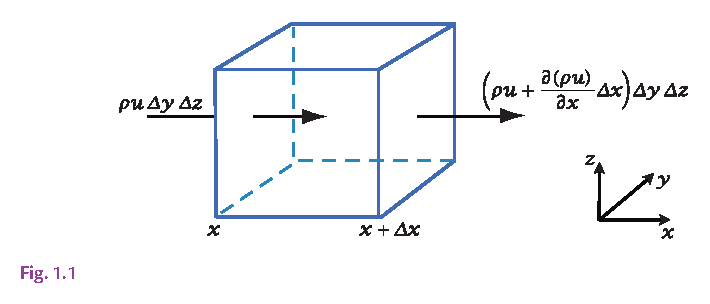
\includegraphics[width=0.8\textwidth]{assets/fig_continuity1.pdf}
  \caption{
    Mass conservation in an rectangular Eulerian control volume.
    The mass convergence, $\partial(\rho u)/\partial x$
    (plus contributions in the $y$ and $z$ directions),
    must be balanced by a density decrease.
    This is Fig. 1.1 in AOFD (Vallis, 2017).
  }
  \label{fig:continuity1}
\end{figure}

\begin{equation}
  \int_V \frac{\partial \rho}{\partial t} dV =
  \rho u + \frac{\partial (\rho u)}{\partial x} \Delta x) \Delta y \Delta z - \rho u \Delta y \Delta z =
\end{equation}

\begin{equation}
  \int_V \frac{\partial \rho}{\partial t} dV =
  \frac{\partial (\rho u)}{\partial x} \Delta x \Delta y \Delta z
\end{equation}
Now, we we allow a flow field to have components in the $y$ and $z$ directions,
the equation becomes:

\begin{equation}
  \int_V \frac{\partial \rho}{\partial t} dV =
  \left[\frac{\partial (\rho u)}{\partial x} + \frac{\partial (\rho v)}{\partial y} + \frac{\partial (\rho w)}{\partial z} \right] \Delta V
\end{equation}
Let $\Delta V \to 0$ to such that any field within $\Delta V$ is uniform to obtain:

\begin{equation}
  \frac{\partial \rho}{\partial t} + \nabla \cdot (\rho \mathbf{u}) = 0
  \label{eq:continuity_eulerian}
\end{equation}
This is the continuity equation in the Eulerian reference frame.

We're not constrained to a rectangular, fixed volume, however.
We can derive this equation for an arbitrary control volume using the divergence
theorem.
The total rate of change of that volume as it moves with the fluid is equal to
the surface integral of the velocity field $\mathbf{u}$ through the surface
$S$ that is bounding the volume $V$ (Fig. \ref{fig:continuity2}).
Mathematically, we can express this as:

\begin{figure}[h]
  \centering
  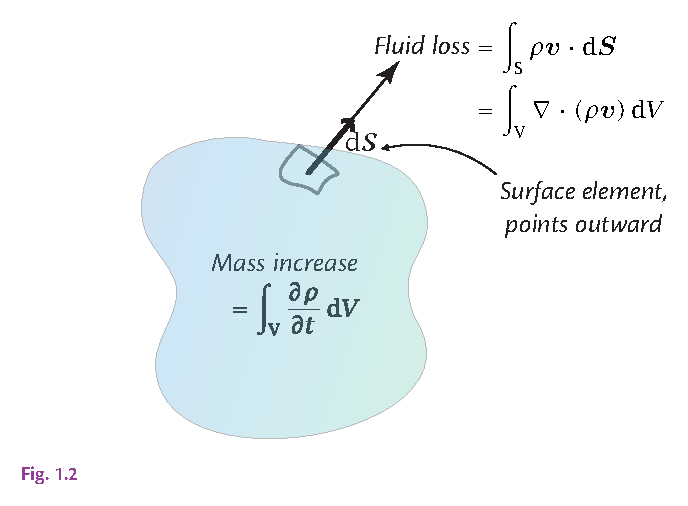
\includegraphics[width=0.7\textwidth]{assets/fig_continuity2.pdf}
  \caption{
    Mass conservation in an arbitrary Eulerian control volume $V$ bounded by a
    surface $S$. The mass increase, $\int_V(\partial \rho/\partial t)dV$
    is equal to the mass flowing into the volume,
    $-\int_S(\rho\mathbf{v}) \cdot d\mathbf{S} = -\int_V \nabla \cdot (\rho\mathbf{v})dV$.
    This is Fig. 1.2 in AOFD (Vallis, 2017).
  }
  \label{fig:continuity2}
\end{figure}

\begin{equation}
  \int_V \frac{\partial \rho}{\partial t} dV = \int_S \rho \mathbf{u} \cdot d\mathbf{S}
\end{equation}
Now, recall the divergence theorem (Eq. \ref{eq:divergence_theorem}) to obtain:

\begin{equation}
  \int_V \frac{\partial \rho}{\partial t} dV = \int_V \nabla \cdot (\rho \mathbf{u}) dV
\end{equation}
Let $\Delta V \to 0$ to integrate and drop $\Delta V$ on both sides to obtain
Eq. \ref{eq:continuity_eulerian}, which is the Eulerian form of the continuity
equation.

\subsubsection{Lagrangian derivation}
\index{Continuity!Lagrangian derivation}

In the Lagrangian frame, we follow a fluid parcel as it moves through space.
Its mass $\rho \Delta V$ is constant by definition, but its density or volume
may change.
Since the mass of the parcel is constant, its Lagrangian derivative is zero:

\begin{equation}
  \frac{d}{dt} (\rho \Delta V) = 0
\end{equation}
Since the mass doesn't change, any change in the density of the parcel must be
balanced by a change in its volume:

\begin{equation}
  \Delta V \frac{d\rho}{dt} + \rho \frac{d\Delta V}{dt} = 0
\end{equation}
Recall that we've already derived the Lagrangian derivative of a volume of the
fluid parcel (Eq. \ref{eq:lagrangian_volume_derivative}), which is the second
term here.
The equation becomes:

\begin{equation}
  \Delta V \frac{d\rho}{dt} + \Delta V \rho \nabla \cdot \mathbf{u} = 0
\end{equation}
Finally, drop $\Delta V$ on both sides to obtain the Lagrangian form of the
continuity equation:

\begin{equation}
  \frac{d\rho}{dt} + \rho \nabla \cdot \mathbf{u} = 0
  \label{eq:continuity_lagrangian}
\end{equation}

Equations \ref{eq:continuity_eulerian} and \ref{eq:continuity_lagrangian} are
two fundamental expressions of the conservation of mass for a fluid.
In one form or another, this equation is a critical component of all weather,
ocean, and climate prediction models.

\subsubsection{Continuity of an incompressible fluid}

Liquids are nearly incompressible, and for them $\frac{d\rho}{dt} = 0$ is a good
approximation.
For an incompressible fluid, the continuity equation simplifies to:

\begin{equation}
  \nabla \cdot \mathbf{u} = 0
  \label{eq:continuity_incompressible}
\end{equation}
Although as simple as it gets, Eq. \ref{eq:continuity_incompressible} is
extremely important in fluid dynamics.

\subsection{Conservation of momentum}

Like the conservation of mass, the conservation of momentum is a fundamental
concept in fluid mechanics.
It allows us to predict how the fluid should accelerate due to its state
(i.e. velocity and density) and due to the forces acting on it.
Together, the continuity and momentum conservation
equations form the core of most fluid prediction models, such as weather, ocean,
and climate prediction models.
We will derive the momentum equation in the remainder of this section.
We'll start from the most basic form first and then incrementally introduce
some common forces, such as the pressure gradient force, gravity, and viscosity.

\subsubsection{The first step}

To derive the momentum conservation equation, we will start from the second
Newton's law, which states that the time rate of change of the momentum of a
fluid particle is equal to the net force acting on it.
For a fluid parcel of volume $\Delta V = \int_V dV$ whose momentum per unit mass
is $\rho \mathbf{u}$, the momentum conservation equation is:

\begin{equation}
  \frac{d}{dt} \int_V \rho \mathbf{u} dV = \int_V \mathbf{F} dV
\end{equation}
where $\mathbf{F}$ is the net force per unit volume acting on the fluid parcel.
Let again the volume parcel be very small such that its density and net force
acting on it are uniform. We have:

\begin{equation}
  \rho \frac{d\mathbf{u}}{dt} \Delta V = \mathbf{F} \Delta V
\end{equation}

\begin{equation}
  \rho \frac{d\mathbf{u}}{dt} = \mathbf{F}
\end{equation}
Recall the Lagrangian derivative operator from Eq. \ref{eq:lagrangian_derivative}
to obtain:

\begin{equation}
  \frac{\partial \mathbf{u}}{\partial t} + (\mathbf{u} \cdot \nabla) \mathbf{u} = \frac{\mathbf{F}}{\rho}
  \label{eq:momentum_eulerian}
\end{equation}
This equation states that the acceleration of a fluid parcel at any fixed point
in space is equal to the net force per unit mass acting on it, divided by the
fluid density.
The second term on the left-hand side is the \textit{advection term}\index{Advection}.
It represents the local acceleration of the fluid parcel due to the properties
of the fluid flow itself.
Consider for example a 1-dimensional flow such that the advection term reduces
to $u \frac{\partial u}{\partial x}$.
Notice that the advection term is zero only in two special cases:
when the velocity is zero or when the velocity is spatially uniform.
In all other cases the advection term is non-zero and contributes to the local
acceleration.

Because the advection term is velocity multiplied by its gradient, it is
\textit{nonlinear}\index{Nonlinear}.
This single property of this term makes accurate analysis and prediction of
fluid flows difficult.
For example, the nonlinear advection term is responsible for the existence of
\textit{chaos}\index{Chaos} in fluid flows, where small differences in initial
conditions lead to vastly different outcomes (in popular culture known as the
\textit{butterfly effect}).
One consequence of this in our daily lives is that weather predictability
is limited to a finite lead time horizon, for example one to two weeks depending
on the weather patterns of interest.
If, however, we could assume that either the velocity or its gradient are so
small that they could be neglected, the equation simplifies significantly
and often allows for analytical solutions.

Back to our equation now.
For a 3-dimensional Cartesian flow where the velocity field is $\mathbf{u} = (u, v, w)$
and net forces are $\mathbf{F} = (F_x, F_y, F_z)$, Eq. \ref{eq:momentum_eulerian}
becomes a system of three equations, one for each component of the velocity field.
Recall from the Lagrangian derivative operator that $(\mathbf{u} \cdot \nabla) \mathbf{u}$
is an operator acting on $\mathbf{u}$ (as opposed to divergence of a gradient).
The $(\mathbf{u} \cdot \nabla)$ operator then expands to
$u\frac{\partial}{\partial x} + v\frac{\partial}{\partial y} + w\frac{\partial}{\partial z}$.
Our vector equations becomes a system of three scalar equations:

\begin{equation}
  \frac{\partial u}{\partial t} + u \frac{\partial u}{\partial x} + v \frac{\partial u}{\partial y} + w \frac{\partial u}{\partial z} = \frac{F_x}{\rho}
\end{equation}

\begin{equation}
  \frac{\partial v}{\partial t} + u \frac{\partial v}{\partial x} + v \frac{\partial v}{\partial y} + w \frac{\partial v}{\partial z} = \frac{F_y}{\rho}
\end{equation}

\begin{equation}
  \frac{\partial w}{\partial t} + u \frac{\partial w}{\partial x} + v \frac{\partial w}{\partial y} + w \frac{\partial w}{\partial z} = \frac{F_z}{\rho}
\end{equation}
Each of the prognostic equations for the velocity components thus has exactly
three advective components that correspond to the gradients of the velocity
in each respective direction.

\subsubsection{Incorporating the forces}

Now we should consider what forces may be acting on the fluid.
We distinguish between two types of forces: surface forces and body forces.
Surface forces act on the surface of the fluid parcel due to the motion of the
fluid molecules, in all directions at that surface.
For example, organized motion of molecules into the surface may cause pressure
on that surface, and the sheared motion of molecules (e.g. if flow is
antiparallel to the surface) may cause shear stress on the surface, leading to
the deformation of the fluid parcel.
In contrast, body forces act remotely (meaning, from a distance) on the entire
volume of the fluid parcel because that parcel is immersed in one or more force fields.
Gravity is one such body force, and it's the only one we'll consider here.
Although in Eq. \ref{eq:momentum_eulerian} we wrote the net force as $\mathbf{F}$,
it's useful to write it as the sum of body forces $\mathbf{F}_b$ and surface
forces $\mathbf{F}_s$:

\begin{equation}
  \frac{\partial \mathbf{u}}{\partial t} + (\mathbf{u} \cdot \nabla) \mathbf{u} = \frac{1}{\rho} (\mathbf{F}_s + \mathbf{F}_b)
\end{equation}

Let's derive the surface forces first.
We want to find out the local change of momentum only due to the surface forces.
Analogous to how the flow through the volume determined the rate of change of
density inside that volume, as we saw in the continuity equation
(Eq. \ref{eq:continuity_eulerian}), the change in momentum inside the volume
is determined by the surface forces acting on the volume (Fig. \ref{fig:momentum1}).

\begin{figure}[h]
  \centering
  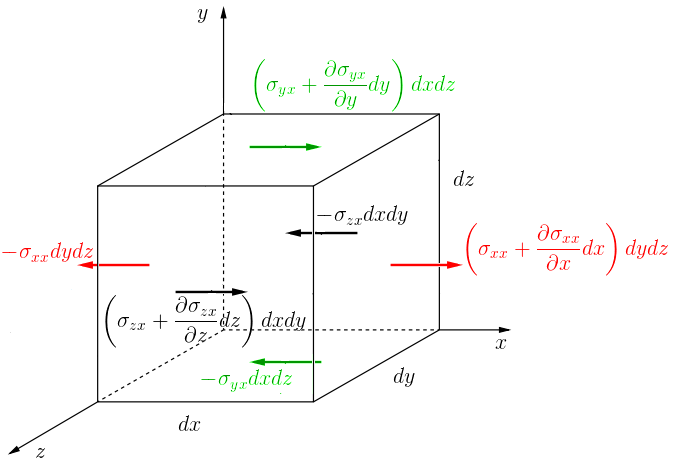
\includegraphics[width=0.8\textwidth]{assets/fig_momentum1.png}
  \caption{
    Normal components of the stress tensor $\mathbf{\sigma}$ acting on a fluid parcel.
    Reproduced from \url{https://en.wikipedia.org/wiki/Cauchy_momentum_equation}
    under the CC BY-SA 4.0 license.
  }
  \label{fig:momentum1}
\end{figure}

Mathematically, we can express this change as:

\begin{equation}
  \int_V \mathbf{F_s} dV = \int_S \boldsymbol{\sigma} \cdot d\mathbf{S}
\end{equation}
where $\boldsymbol{\sigma}$ is the second-order stress tensor acting on the
surface $S$ of the fluid parcel.
As before, recall the divergence theorem (Eq. \ref{eq:divergence_theorem}) to obtain:

\begin{equation}
  \int_V \mathbf{F_s} dV = \int_V \nabla \cdot \boldsymbol{\sigma} dV
\end{equation}

\begin{equation}
  \mathbf{F_s} = \nabla \cdot \boldsymbol{\sigma}
\end{equation}
The surface force thus equals the divergence of the stress tensor.
Insert this into Eq. \ref{eq:momentum_eulerian} to get our new form of
the momentum equation:

\begin{equation}
  \frac{\partial \mathbf{u}}{\partial t} + (\mathbf{u} \cdot \nabla) \mathbf{u} =
  \frac{1}{\rho} \nabla \cdot \boldsymbol{\sigma} + \frac{\mathbf{F}_b}{\rho}
\end{equation}
This form of the momentum equation is often called the
\textit{Cauchy momentum equation}\index{Momentum equation!Cauchy}.

Let's now look at what this stress tensor divergence term
$\nabla \cdot \boldsymbol{\sigma}$ is.

\subsubsection{Pressure gradient}

There is a fundamental difference in the meaning of the diagonal and off-diagonal
components of the stress tensor.
The diagonal components of the stress tensor, $\sigma_{xx}$, $\sigma_{yy}$, and
$\sigma_{zz}$, represent the normal stress components, i.e. the force per unit
area acting on a surface element that is oriented in the $x$, $y$, and $z$
directions, respectively.
The off-diagonal components of the stress tensor represent the shear stress
components, each acting on all three surfaces.
For example, $\sigma_{xy}$ represents the $x$-component of the stress tensor
acting on the surface that is perpendicular to the $y$-axis.
Let's write out the stress tensor in Cartesian coordinates:

\begin{equation}
  \boldsymbol{\sigma} = \begin{bmatrix}
    \sigma_{xx} & \sigma_{xy} & \sigma_{xz} \\
    \sigma_{yx} & \sigma_{yy} & \sigma_{yz} \\
    \sigma_{zx} & \sigma_{zy} & \sigma_{zz}
  \end{bmatrix}
\end{equation}

This tensor can be decomposed into its normal and shear components:

\begin{equation}
  \boldsymbol{\sigma} = -p \mathbf{I} + \boldsymbol{\tau}
  \label{eq:stress_tensor_decomposition}
\end{equation}
where $p$ is the pressure, $\mathbf{I}$ is the identity tensor\index{Tensor!Identity},
and $\boldsymbol{\tau}$ is the deviatoric stress tensor, or, the viscous shear
stress tensor\index{Stress!Shear}.
Written out explicitly in Cartesian coordinates and using Eq.
\ref{eq:stress_tensor_decomposition}, the stress tensor is:

\begin{equation}
  \boldsymbol{\sigma} = \begin{bmatrix}
    -p + \tau_{xx} & \tau_{xy} & \tau_{xz} \\
    \tau_{yx} & -p + \tau_{yy} & \tau_{yz} \\
    \tau_{zx} & \tau_{zy} & -p + \tau_{zz}
  \end{bmatrix}
\end{equation}

The divergence of the stress tensor is then:

\begin{equation}
  \nabla \cdot \boldsymbol{\sigma} = - \nabla p + \nabla \cdot \boldsymbol{\tau}
\end{equation}
Let's insert this into Eq. \ref{eq:momentum_eulerian} to get our new form of
the momentum equation:

\begin{equation}
  \frac{\partial \mathbf{u}}{\partial t} + (\mathbf{u} \cdot \nabla) \mathbf{u} =
  - \frac{1}{\rho} \nabla p + \frac{1}{\rho} \nabla \cdot \boldsymbol{\tau} + \frac{\mathbf{F}_b}{\rho}
  \label{eq:momentum_cauchy_with_shear}
\end{equation}

Pressure is one of the fluid properties that determine its state.
Collective, organized, motion of molecules at a macroscopic scale induces
pressure on a surface and an associated force acting normal to that surface.
Recall that the surface vector is normal to the surface and pointing outward,
and the force acting on the fluid surface is oriented inward, thus the minus sign.

In an ideal, \textit{inviscid} fluid, that is, a fluid that exhibits no viscous
forces, the stress tensor $\boldsymbol{\sigma}$ is only composed of the diagonal
terms (pressure), and the divergence of the stress tensor is zero.
Dropping $\nabla \cdot \boldsymbol{\tau}$ and the body forces $\mathbf{F}_b$ for
now, the Cauchy momentum equation simplifies to:

\begin{equation}
  \frac{\partial \mathbf{u}}{\partial t} + (\mathbf{u} \cdot \nabla) \mathbf{u} =
  - \frac{1}{\rho} \nabla p
  \label{eq:momentum_euler}
\end{equation}
This form of the momentum equation is often called the \textit{Euler equation}.
\index{Momentum equation!Euler}

\subsubsection{Viscous forces}

Now, let's look at the shear stress tensor divergence $\nabla \cdot \boldsymbol{\tau}$.
Written out explicitly as a matrix of all its components, $\boldsymbol{\tau}$ is:

\begin{equation}
  \boldsymbol{\tau} = \begin{bmatrix}
    \tau_{xx} & \tau_{xy} & \tau_{xz} \\
    \tau_{yx} & \tau_{yy} & \tau_{yz} \\
    \tau_{zx} & \tau_{zy} & \tau_{zz}
  \end{bmatrix}
\end{equation}
The diagonal components of the deviatoric stress tensor are the normal stresses,
while the off-diagonal components are the shear stresses.
The normal stresses are non-zero only in compressible fluids ($\nabla \cdot \mathbf{u} \neq 0$),
while the shear stresses are zero in non-viscous flows.
The divergence of this tensor, written out explicitly as a matrix of all its
components, is:

\begin{equation}
  \nabla \cdot \boldsymbol{\tau} = \begin{bmatrix}
    \frac{\partial \tau_{xx}}{\partial x} + \frac{\partial \tau_{yx}}{\partial y} + \frac{\partial \tau_{zx}}{\partial z} \\
    \frac{\partial \tau_{xy}}{\partial x} + \frac{\partial \tau_{yy}}{\partial y} + \frac{\partial \tau_{zy}}{\partial z} \\
    \frac{\partial \tau_{xz}}{\partial x} + \frac{\partial \tau_{yz}}{\partial y} + \frac{\partial \tau_{zz}}{\partial z}
  \end{bmatrix}
\end{equation}

Now, write out \ref{eq:momentum_cauchy_with_shear} as a system of three scalar
equations, one for each component of the velocity field, and insert the shear
stress divergence terms to get:

\begin{equation}
  \frac{\partial u}{\partial t} + 
  u \frac{\partial u}{\partial x} + 
  v \frac{\partial u}{\partial y} + 
  w \frac{\partial u}{\partial z} = 
  - \frac{1}{\rho} \frac{\partial p}{\partial x} + 
  \frac{1}{\rho} \left( \frac{\partial \tau_{xx}}{\partial x} + \frac{\partial \tau_{yx}}{\partial y} + \frac{\partial \tau_{zx}}{\partial z} \right) + 
  \frac{F_x}{\rho}
\end{equation}

\begin{equation}
  \frac{\partial v}{\partial t} + 
  u \frac{\partial v}{\partial x} + 
  v \frac{\partial v}{\partial y} + 
  w \frac{\partial v}{\partial z} = 
  - \frac{1}{\rho} \frac{\partial p}{\partial y} + 
  \frac{1}{\rho} \left( \frac{\partial \tau_{xy}}{\partial x} + \frac{\partial \tau_{yy}}{\partial y} + \frac{\partial \tau_{zy}}{\partial z} \right) + 
  \frac{F_y}{\rho}
\end{equation}

\begin{equation}
  \frac{\partial w}{\partial t} + 
  u \frac{\partial w}{\partial x} + 
  v \frac{\partial w}{\partial y} + 
  w \frac{\partial w}{\partial z} = 
  - \frac{1}{\rho} \frac{\partial p}{\partial z} + 
  \frac{1}{\rho} \left( \frac{\partial \tau_{xz}}{\partial x} + \frac{\partial \tau_{yz}}{\partial y} + \frac{\partial \tau_{zz}}{\partial z} \right) + 
  \frac{F_z}{\rho}
\end{equation}
Each of the prognostic equations for the velocity components thus has exactly
one pressure gradient and two shear stress gradient terms, all arising from the
surface forces.

Experimentally, it was found that the viscous shear stress tensor $\boldsymbol{\tau}$
is proportional to the gradient of the velocity field, i.e. $\boldsymbol{\tau} = \mu \nabla \mathbf{u}$.
This property of the fluid makes it a so-called \textit{Newtonian fluid}\index{Fluid!Newtonian}.
The proportionality constant $\mu$ is the dynamic viscosity and depends on the
fluid properties and temperature.
Inserting this into Eq. \ref{eq:momentum_cauchy_with_shear} and assuming
incompressibility, we get:

\begin{equation}
  \frac{\partial \mathbf{u}}{\partial t} + (\mathbf{u} \cdot \nabla) \mathbf{u} =
  - \frac{1}{\rho} \nabla p + \frac{1}{\rho} \nabla \cdot (\mu \nabla \mathbf{u}) +
  \frac{\mathbf{F}_b}{\rho}
\end{equation}
We can further simplify this equation by assuming that the viscosity is constant
and that the flow is incompressible.
This allows us to neglect the viscous stress gradient term, leading to the
\textit{Navier-Stokes equation}\index{Momentum equation!Navier-Stokes}.

\begin{equation}
  \frac{\partial \mathbf{u}}{\partial t} + (\mathbf{u} \cdot \nabla) \mathbf{u} =
  - \frac{1}{\rho} \nabla p + \nu \nabla^2 \mathbf{u} +
  \frac{\mathbf{F}_b}{\rho}
  \label{eq:momentum_navier_stokes}
\end{equation}
where $\nu = \frac{\mu}{\rho}$ is the kinematic viscosity.
The $\nabla^2$ operator is often called the \textit{Laplacian}\index{Laplacian}.
It is a second-order differential operator that appears in many partial
differential equations, including the heat equation, the wave equation, and
the Laplace equation.
More on these later.

Let's now look at the body forces to conclude our derivation.

\subsubsection{Gravity}

As we mentioned earlier, gravity is the only body force we'll consider here.
The force of gravity per unit mass is given by $\mathbf{g} = (0, 0, -g)$,
where $g$ is the gravitational acceleration.
Here we're assuming that the gravitational acceleration is constant and always
points downward.
Insert this into Eq. \ref{eq:momentum_navier_stokes} and assuming
incompressibility, we get:

\begin{equation}
  \frac{\partial \mathbf{u}}{\partial t} + (\mathbf{u} \cdot \nabla) \mathbf{u} =
  - \frac{1}{\rho} \nabla p + \mathbf{g} + \nu \nabla^2 \mathbf{u}
\end{equation}

Written out explicitly, we get:

\begin{equation}
  \frac{\partial u}{\partial t} + 
  u \frac{\partial u}{\partial x} + 
  v \frac{\partial u}{\partial y} + 
  w \frac{\partial u}{\partial z} = 
  - \frac{1}{\rho} \frac{\partial p}{\partial x} + \nu \left( \frac{\partial^2 u}{\partial x^2} + \frac{\partial^2 u}{\partial y^2} + \frac{\partial^2 u}{\partial z^2} \right)
\end{equation}

\begin{equation}
  \frac{\partial v}{\partial t} + 
  u \frac{\partial v}{\partial x} + 
  v \frac{\partial v}{\partial y} + 
  w \frac{\partial v}{\partial z} = 
  - \frac{1}{\rho} \frac{\partial p}{\partial y} + \nu \left( \frac{\partial^2 v}{\partial x^2} + \frac{\partial^2 v}{\partial y^2} + \frac{\partial^2 v}{\partial z^2} \right)
\end{equation}

\begin{equation}
  \frac{\partial w}{\partial t} + 
  u \frac{\partial w}{\partial x} + 
  v \frac{\partial w}{\partial y} + 
  w \frac{\partial w}{\partial z} = 
  - \frac{1}{\rho} \frac{\partial p}{\partial z} - g + \nu \left( \frac{\partial^2 w}{\partial x^2} + \frac{\partial^2 w}{\partial y^2} + \frac{\partial^2 w}{\partial z^2} \right)
  \label{eq:momentum_navier_stokes_scalar_w}
\end{equation}
This completes the full system of momentum conservation equations in the
Cartesian coordinate system.

\subsection{Hydrostatic balance}

Take Eq. \ref{eq:momentum_navier_stokes_scalar_w} and assume that the vertical
acceleration $\frac{dw}{dt}$ is small compared to $g$, and that the spatial
variations of $w$ are small.
We can then drop the $\frac{dw}{dt}$ and $\nu \nabla^2 w$ terms to get the
\textit{hydrostatic approximation}\index{Hydrostatic approximation}:

\begin{equation}
  \frac{\partial p}{\partial z} = - \rho g
  \label{eq:hydrostatic_approximation}
\end{equation}
which states that the vertical pressure gradient is governed by the density
of the fluid and the gravitational acceleration.
It's often a good approximation for large-scale atmospheric and oceanic flows,
where the vertical variations of the horizontal velocity components are much
smaller than the horizontal variations of the vertical velocity component.
Notice however that the hydrostatic approximation does not imply that there
is no vertical motion or that it does not vary over time.
Instead, according to the continuity equation (Eq. \ref{eq:continuity_lagrangian}),
it means that the vertical motion is completely governed by the change in
density and the divergence of the horizontal velocity field.
Further, if the flow is incompressible ($\nabla \cdot \mathbf{u} = 0$),
we get:

\begin{equation}
  \frac{\partial w}{\partial z} = - \frac{\partial u}{\partial x} - \frac{\partial v}{\partial y}
  \label{eq:hydrostatic_continuity}
\end{equation}
This relationship will prove to be extremely useful in ocean applications where
only the horizontal velocity field is resolved.
For example, a group of ocean surface drifters converging towards a region is
indicative of downwelling (downward motion in the ocean) in that region.
Another example is that of ocean circulation models, which are typically
designed as hydrostatic.
In the case of such models, the horizontal components of the velocity are
prognostic variables, and the vertical velocity is diagnosed using
Eq. \ref{eq:hydrostatic_continuity}.

\subsection{Equation of state}

Now that we have derived the mass and momentum conservation equations, let's
write them out together in vector form:

\begin{equation}
  \frac{\partial \mathbf{u}}{\partial t} + (\mathbf{u} \cdot \nabla) \mathbf{u} =
  - \frac{1}{\rho} \nabla p + \mathbf{g} + \nu \nabla^2 \mathbf{u}
  \label{eq:momentum_navier_stokes_state}
\end{equation}

\begin{equation}
  \frac{\partial \rho}{\partial t} + \nabla \cdot (\rho \mathbf{u}) = 0
  \label{eq:continuity_eulerian_state}
\end{equation}
Momentum and mass conservation equations are prognostic equations for the
vector velocity field $\mathbf{u}$ and the scalar density field $\rho$,
respectively.
Notice the one remaining unknown: the scalar pressure field $p$.
As of now, we have a system of two independent equations for the three unknowns:
$\mathbf{u}$, $p$, and $\rho$.
We need one more equation to close the system---the
\textit{equation of state}\index{Equation of state}---to relate the pressure to
the other properties of the fluid, such as temperature, density, and
composition.

The prognostic equations that we have derived so far describe equally well
the evolution of both the atmosphere and the ocean, despite their significant
differences.
The equation of state is where our systems of governing equations for the ocean
and the atmosphere begin to diverge.
Namely, the atmosphere is a mixture of dry air and water vapor, and the
ocean is composed of liquid water with varying amounts of dissolved salts.
These differences will reflect in the choice of the equation of state to use
in each of these systems.

\subsubsection{In the atmosphere}

In the atmospheres, \textit{ideal gas law}\index{Equation of state!Ideal gas law}
is often used as the equation of state:

\begin{equation}
  p = \rho R T
  \label{eq:ideal_gas_law}
\end{equation}
where $R$ is the specific gas constant for the gas in question, and $T$ is the
temperature.
For the moist air, we need account for both the properties of dry air
($R_d \approx 287 J kg^{-1} K^{-1}$) and those of water vapor
($R_v \approx 461 J kg^{-1} K^{-1}$).
The equation of state for moist air relies on the so-called
\textit{virtual temperature}\index{Virtual temperature} to account for the
moisture in the air:

\begin{equation}
  p = \rho R_d T_v
\end{equation}
where:

\begin{equation}
  T_v = T \left[1 + q \left(\frac{R_v}{R_d} - 1 \right) \right]
\end{equation}
where $q$ is the specific humidity of the air.
So, the equation of state for moist air is:

\begin{equation}
  p = \rho R_d T \left[1 + q \left(\frac{R_v}{R_d} - 1 \right) \right]
  \label{eq:equation_of_state_atmosphere}
\end{equation}

Recall that we intended to close our system of equations by finding the
equation for pressure.
Although we did solve for pressure, it seems that we introduced two new
unknown variables: the temperature $T$ and the specific humidity $q$.
Each of these variables are governed by their own conservation equations,
akin to that for density, but with the addition of source and sink terms
that control their production and loss:

\begin{equation}
  \frac{\partial T}{\partial t} + (\mathbf{u} \cdot \nabla) T = \dot{S}_T
  \label{eq:temperature_equation}
\end{equation}

\begin{equation}
  \frac{\partial q}{\partial t} + (\mathbf{u} \cdot \nabla) q = \dot{S}_q
  \label{eq:specific_humidity_equation}
\end{equation}
where $\dot{S}_T$ and $\dot{S}_q$ are the sources and sinks of temperature and
specific humidity, respectively.

Although we won't delve further into the details behind the sources and sinks
of temperature and specific humidity in the atmosphere, we can denote these
equations as completing the full system of prognostic equations for the
atmosphere: Eqs. \ref{eq:momentum_navier_stokes_state}, 
\ref{eq:continuity_eulerian_state},
\ref{eq:equation_of_state_atmosphere},
\ref{eq:temperature_equation}, and
\ref{eq:specific_humidity_equation}.
These equations form the basis of many weather and climate prediction models.

\subsubsection{In the ocean}

Ideal gas law (Eq. \ref{eq:ideal_gas_law}) doesn't apply to liquids and the
equation of state for seawater is not easily derived.
Instead, we assume that the ocean is a single-component fluid, and we use the
density field $\rho$ as the equation of state.

\begin{equation}
  \rho = \rho(T, S, p) \\
  = \rho_0 \left[ 1 - \beta_T(T-T_0) + \beta_S(S-S_0) + \beta_p(p-p_0) \right]
  \label{eq:equation_of_state_ocean}
\end{equation}
where $\rho_0$ is the reference density at the reference temperature $T_0$,
salinity $S_0$, and pressure $p_0$.
The coefficients $\beta_T$, $\beta_S$, and $\beta_p$ are the thermal expansion
coefficient, the saline contraction coefficient, and the pressure
coefficient, respectively.
This form of the equation of state is a linear equation of state (as in, the
dependence of density on temperature, salinity, and pressure each is linear).
Dependence of density on temperature and salinity at two different pressure
levels is shown in Fig. \ref{fig:seawater_eqstate}.
Higher order equations of state are often used for higher accuracy, however
they're out of scope for this course.

\begin{figure}[h]
  \centering
  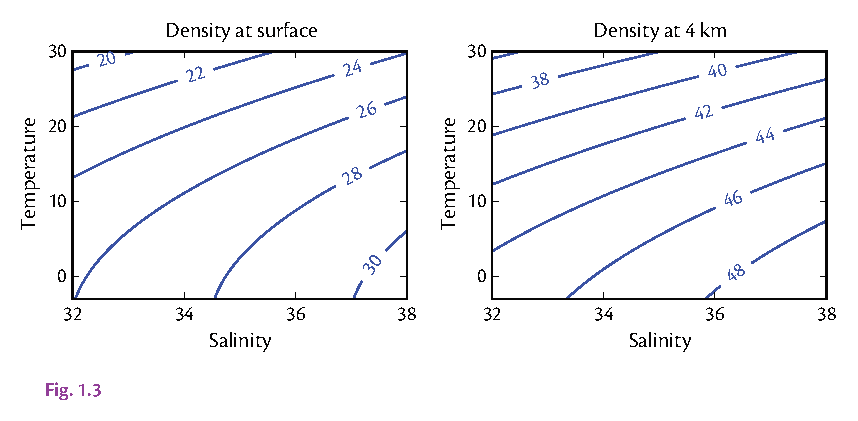
\includegraphics[width=\textwidth]{assets/fig_seawater_eqstate.pdf}
  \caption{
    Contours of density as a function of temperature and salinity for seawater.
    Contour labels are (density - 1000) kg m$^{-3}$.
    Left panel: at sea-level ($p = 10^5\ Pa$, or 1000 mb).
    Right panel: at $p = 4 \times 10^7\ Pa$ (about 4 km depth).
    In both cases the contours are slightly convex, so that if two parcels at
    the same density but different temperatures and salinities are mixed, the
    resulting parcel is of higher density.
    (The average temperature is not exactly conserved on mixing, but it very
    nearly is.)
    This is Fig. 1.3 in AOFD (Vallis, 2017).
  }
  \label{fig:seawater_eqstate}
\end{figure}

Like we did in the case of atmosphere, here we need to additional prognostic
equations, one of temperature and another for salinity:

\begin{equation}
  \frac{\partial T}{\partial t} + (\mathbf{u} \cdot \nabla) T = \dot{S}_T
  \label{eq:temperature_equation_ocean}
\end{equation}

\begin{equation}
  \frac{\partial S}{\partial t} + (\mathbf{u} \cdot \nabla) S = \dot{S}_S
  \label{eq:salinity_equation_ocean}
\end{equation}
where $\dot{S}_T$ and $\dot{S}_S$ are the sources and sinks of water temperature
and salinity, respectively.

Equations \ref{eq:momentum_navier_stokes_state},
\ref{eq:continuity_eulerian_state},
\ref{eq:equation_of_state_ocean},
\ref{eq:temperature_equation_ocean}, and
\ref{eq:salinity_equation_ocean} are the governing equations used in most
numerical ocean circulation models.

\subsection{Nondimensionalization and scaling}
\label{sec:nondimensionalization_and_scaling}

A useful technique to simplify the analysis of the governing equations is to
scale the variables using characteristic values for each of the variables.
This is known as \textit{nondimensionalization}\index{Nondimensionalization}
or \textit{scaling the equations}\index{Scaling}.
In practice, for each (dependent or independent) variable $x$ in the equations,
we define a characteristic value $X$.
For example, for the velocity $\mathbf{u}$, we may pick the characteristic
value of $U = 1\ m\ s^{-1}$ or $U = 10\ m\ s^{-1}$ for the ocean or atmosphere,
respectively.
We then divide each term in the equations by the characteristic value to
obtain a nondimensional (unitless) number.
This helps us identify the important parameters that govern the behavior of
the system and to group terms in the equations that are of similar magnitudes.
This is especially useful for large-scale flows, where the length and time
scales can vary over several orders of magnitude.

For example, let's look at the vector equation for horizontal momentum
(thus, ignoring $\mathbf{g}$ for now):

\begin{equation}
  \frac{\partial \mathbf{u}}{\partial t} + (\mathbf{u} \cdot \nabla) \mathbf{u} =
  - \frac{1}{\rho} \nabla p + \nu \nabla^2 \mathbf{u}
\end{equation}

The characteristic scales for each term are:

\begin{equation}
  \frac{\partial \mathbf{u}}{\partial t} \sim \frac{U}{T}
\end{equation}

\begin{equation}
  (\mathbf{u} \cdot \nabla) \mathbf{u} \sim \frac{U^2}{L}
\end{equation}

\begin{equation}
  - \frac{1}{\rho} \nabla p \sim \frac{1}{\rho} \frac{P}{L}
\end{equation}

\begin{equation}
  \nu \nabla^2 \mathbf{u} \sim \nu \frac{U}{L^2}
\end{equation}
where $U$, $T$, $L$, and $P$ are the characteristic scales for the velocity,
time, length, and pressure, respectively.
So, if for a given flow we can estimate these characteristic values, we can
easily determine which terms are important and which can be neglected.
This is the basis of scaling arguments in fluid mechanics.

This approach also enables characterizing the flows in terms of
nondimensional numbers.
For example, to describe how turbulent or laminar a flow is, it's useful to
relate the inertial to the viscous terms in the momentum equation.
Their ratio is called the  \textit{Reynolds number}\index{Reynolds number}:

\begin{equation}
  \frac{(\mathbf{u} \cdot \nabla) \mathbf{u}}{\nu \nabla^2 \mathbf{u}} \sim
  \frac{\frac{U^2}{L}}{\frac{\nu U}{L^2}} = \frac{UL}{\nu} \equiv \text{Re}
  \label{eq:reynolds_number}
\end{equation}
You see that the Reynolds number is proportional to the velocity and length
scales each, and inversely proportional to the viscosity.
A larger Reynolds number corresponds to a more turbulent flow.

\subsection{Exercises}

\begin{enumerate}
  \item Derive the Lagrangian form of the continuity equation from
  the Eulerian form and vice versa. What is the key equation that relates the
  two forms?

  \item Write out the Cauchy, Euler, and Navier-Stokes equations in vector form
  and discuss their similarities and differences.
  Give examples of flows that are well described by each of these equations.

  \item Write a computer program that calculates the divergence of a second-order
  tensor in a Cartesian, 3-dimensional coordinate system.

  \item Consider two opposing, horizontal, surface currents along the $x$-axis.
  In the vertical they uniformly span a mixed layer that extends from the
  surface to the depth of 20 meters, with a magnitude of 1 m s$^{-1}$.
  The two currents meet at a stagnation zone that is 100 meters wide.
  Calculate the downwelling velocity at the bottom of the mixed layer.
  Assume $\nabla \cdot \mathbf{u} = 0$, no change in mean sea level, and no
  flow in the $y$-direction.

  \item Write a function in your favorite programming language that takes a
  value of temperature, salinity, and pressure and returns the density of
  seawater. Assume linear dependence of density on temperature, salinity, and
  pressure. Take the thermal expansion coefficient to be $\beta_T = 1.67 \times 10^{-4} K^{-1}$,
  the Haline contraction coefficient to be $\beta_S = 7.8 \times 10^{-4} g\ kg^{-1}$,
  and the compressibility coefficient to be $\beta_p = 4.4 \times 10^{-10} Pa^{-1}$.
  Take the reference density to be $\rho_0 = 1027\ kg\ m^{-3}$, the reference
  temperature to be $T_0 = 283\ K$, the reference salinity to be $S_0 = 35 g\ kg^{-1}$,
  and the reference pressure to be $p_0 = 10^5\ Pa$.
  When you implement your function, calculate the density of seawater for the
  range of temperatures from -2 to 30 degrees Celsius, and salinities from 20 to
  40 g/kg, and plot it as a contour plot as a function of temperature and salinity.
  Make such plots for pressure values of $10^5$, $10^6$, and $10^7$ Pa.

  \item Calculate the Reynolds number for:
  (a) a synoptic-scale mid-latitude cyclone in the atmosphere;
  (b) an mesoscale ocean eddy;
  (c) a river inflow into the ocean;
  (d) a breaking ocean surface wave;
  (e) water flowing through a pipe with a diameter of 0.1 m and flow speed of 1 m s$^{-1}$.
  Assume $\nu = 10^{-5} m^2 s^{-1}$ for air and $\nu = 10^{-6} m^2 s^{-1}$ for water.

\end{enumerate}

\subsection*{Further reading}

\begin{itemize}
  \item Sections 1.2-1.4 of \textit{EAOD} by Vallis
  \item Sections 4.1-4.6 of \textit{Fluid Mechanics} by Kundu, Cohen, and Dowling
\end{itemize}

\newpage
\section{Rotating flows}

Fluids behave somewhat differently when in a rotating reference frame, for
example on the surface of a rotating planet.
In this chapter we explore the effects of rotation on the flow.
We begin by deriving the temporal derivative of a general vector in a rotating
reference frame, and then apply it to find the velocity and acceleration in such
a frame.
From there we derive the centrifugal and Coriolis forces, and discuss their
implications for geophysical flows.

\subsection{Rate of change of a rotating vector}

Before determining the what the velocity and acceleration should appear like
in a rotating reference frame (i.e. on the surface of a rotating planet), we
first need to understand how a vector that is fixed in the rotating frame
appears to change over time to the observer in the inertial (fixed) frame.
To do that, consider a vector $\mathbf{C}$ that rotates around an axis at a
constant angular velocity $\mathbf{\Omega}$ (Fig. \ref{fig:rotating_vector}).
The angular velocity $\mathbf{\Omega}$ is the rate of change of the angle in
the plane that is perpendicular to the axis of rotation, and is thus
$\frac{d\lambda}{dt}$.
A unit vector $\mathbf{m}$ is oriented in the direction of the rate of change
of $\mathbf{C}$, and is perpendicular to both $\mathbf{C}$ and $\mathbf{\Omega}$.
We will assume that $\mathbf{\Omega}$ is constant.
This is a generally good assumption for the rotation rates of planets, at least
on time scales that we are interested in.
A small change in $\mathbf{C}$ can then be expressed as:

\begin{figure}[h]
  \centering
  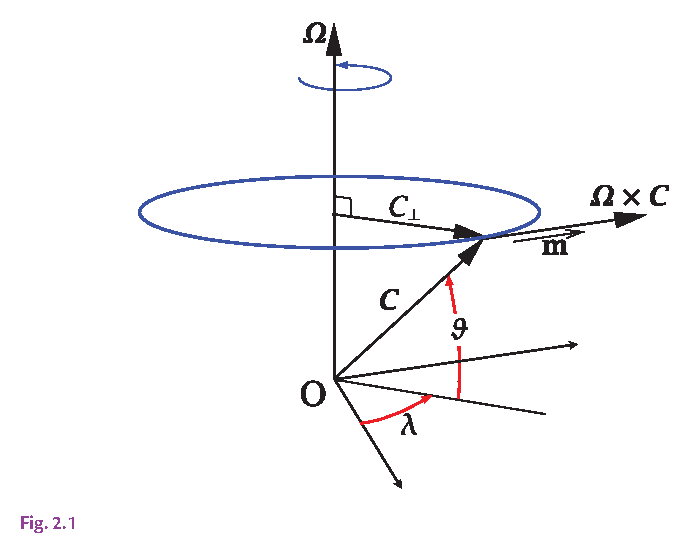
\includegraphics[width=0.8\textwidth]{assets/fig_rotating_vector.pdf}
  \caption{
    A vector $\mathbf{C}$ rotating at an angular velocity $\mathbf{\Omega}$.
    It appears to be a constant vector in the rotating frame, whereas in the
    inertial frame it rotates according to
    $\left(d\mathbf{C}/dt\right)_I = \mathbf{\Omega} \times \mathbf{C}$.
    This is Fig. 2.1 in AOFD (Vallis, 2017).
  }
  \label{fig:rotating_vector}
\end{figure}

\begin{equation}
  \delta \mathbf{C} = |\mathbf{C}| \cos\theta\ \delta \lambda\ \mathbf{m}
\end{equation}
The change in $\mathbf{C}$ is thus proportional to:
its magnitude;
the cosine of the angle between $\mathbf{C}$ and the horizontal plane
(\textit{i.e.} the plane perpendicular to $\mathbf{\Omega}$);
the change in $\lambda$;
and, the unit vector $\mathbf{m}$.
Notice now that using the definition of the cross product (Eq. \ref{eq:cross_product_magnitude}),
we can write the change in $\mathbf{C}$ as:

\begin{equation}
  \delta \mathbf{C} = |\mathbf{C}| |\mathbf{\Omega}| \sin(\pi/2 - \theta)\ \mathbf{m}\ \delta t =
  \mathbf{\Omega} \times \mathbf{C}\ \delta t
\end{equation}
so the rate of change of a rotating vector, when observed from a fixed, inertial
frame is the cross product of the angular velocity and the vector itself:

\begin{equation}
  \left(\frac{d\mathbf{C}}{dt}\right)_I = \mathbf{\Omega} \times \mathbf{C}
\end{equation}
Going forward, we will use the subscript $I$ to denote the inertial frame,
non-rotating reference frame.

Imagine now that you're standing on top of the rotating vector $\mathbf{C}$,
and are still relative to that rotating reference frame, much like standing
still on the surface of a rotating planet.
To you as the observer in the rotating frame, the vector $\mathbf{C}$ appears
to not change in any way.
Consider now another vector $\mathbf{B}$ that may change (in direction or
magnitude, or both) in the rotating reference frame.
We can then say that the rate of change of $\mathbf{B}$ in the inertial frame
is the vector sum of its two rates of change:
The rate of change of $\mathbf{B}$ in the rotating frame, and the rate of
change of the rotating frame itself:

\begin{equation}
  \left(\frac{d\mathbf{B}}{dt}\right)_I = \left(\frac{d\mathbf{B}}{dt}\right)_R + \mathbf{\Omega} \times \mathbf{B}
  \label{eq:rate_of_change_rotating_vector}
\end{equation}

We now have a useful tool to use to determine the velocity and acceleration in
a rotating frame, such as that of of the surface of a rotating planet.

\subsection{Velocity and acceleration in a rotating frame}

Consider now a position vector $\mathbf{r}$ that locates a parcel in the rotating
frame.
The velocity of the parcel in the inertial frame is then given by the rate of
change of the position vector.
Apply Eq. \ref{eq:rate_of_change_rotating_vector} to $\mathbf{r}$ to get:

\begin{equation}
  \left( \frac{d\mathbf{r}}{dt} \right)_I = \left( \frac{d\mathbf{r}}{dt} \right)_R + \mathbf{\Omega} \times \mathbf{r}
\end{equation}
As the time derivative of a position vector is velocity by definition, we can
write this as:

\begin{equation}
  \mathbf{u}_I = \mathbf{u}_R + \mathbf{\Omega} \times \mathbf{r}
  \label{eq:inertial_velocity}
\end{equation}
This relates the inertial and rotating velocities.
Recall that we are interested in accelerations, as it's the acceleration that
we solve for in the Navier-Stokes equations and relate to the forces that act
on the fluid.
We know that the acceleration is the rate of change of velocity, so let's apply
Eq. \ref{eq:rate_of_change_rotating_vector} to the rotating velocity:

\begin{equation}
  \left( \frac{d\mathbf{u}_R}{dt} \right)_I = \left( \frac{d\mathbf{u}_R}{dt} \right)_R + \mathbf{\Omega} \times \mathbf{u}_R
  \label{eq:inertial_acceleration}
\end{equation}
Now, use Eq. \ref{eq:inertial_velocity} to substitute for $\mathbf{u}_I$ in
Eq. \ref{eq:inertial_acceleration}:

\begin{equation}
  \left( \frac{d\left(\mathbf{u}_I - \mathbf{\Omega} \times \mathbf{r}\right)}{dt} \right)_I = 
  \left( \frac{d\mathbf{u}_R}{dt} \right)_R + \mathbf{\Omega} \times \mathbf{u}_R
\end{equation}

\begin{equation}
  \left( \frac{d \mathbf{u}_I}{dt} \right)_I =
  \left( \frac{d \mathbf{u}_R}{dt} \right)_R +
  \mathbf{\Omega} \times \mathbf{u}_R +
  \frac{d\mathbf{\Omega}}{dt} \times \mathbf{r} +
  \mathbf{\Omega} \times \left( \frac{d\mathbf{r}}{dt} \right)_I
  \label{eq:inertial_acceleration_from_rotating}
\end{equation}
Recall that:

\begin{equation}
  \left( \frac{d \mathbf{r}}{dt} \right)_I =
  \left( \frac{d \mathbf{r}}{dt} \right)_R +
  \mathbf{\Omega} \times \mathbf{r} =
  \left( \mathbf{u}_R + \mathbf{\Omega} \times \mathbf{r} \right)
  \label{eq:inertial_velocity_from_rotating}
\end{equation}
If $\mathbf{\Omega}$ is constant, as we have assumed at the beginning,
inserting Eq. \ref{eq:inertial_velocity_from_rotating} into Eq.
\ref{eq:inertial_acceleration_from_rotating} yields:

\begin{equation}
  \left( \frac{d \mathbf{u}_R}{dt} \right)_R =
  \left( \frac{d \mathbf{u}_I}{dt} \right)_I -
  2 \mathbf{\Omega} \times \mathbf{u}_R -
  \mathbf{\Omega} \times \left( \mathbf{\Omega} \times \mathbf{r} \right)
  \label{eq:rotating_acceleration}
\end{equation}

The interpretation of the terms in Eq. \ref{eq:rotating_acceleration} is:

\begin{itemize}
  \item $\left( \frac{d \mathbf{u}_R}{dt} \right)_R$, is the rate of change of
  the relative velocity as observed in the rotating frame.
  This is the rate of change of the velocity that you would measure with an
  anemometer or current meter if position fixed relative to the rotating planet's
  surface. 

  \item $\left( \frac{d \mathbf{u}_I}{dt} \right)_I$, is the rate of change of
  the inertial velocity, \textit{i.e.} the velocity as observed in the inertial
  frame.

  \item $-2 \mathbf{\Omega} \times \mathbf{u}_R$, is the
  \textit{Coriolis acceleration}\index{Coriolis!acceleration}
  \index{Acceleration!Coriolis}.
  The Coriolis acceleration (and correspondingly, the Coriolis force) is
  responsible for the organized rotation of large-scale atmospheric and oceanic
  flows.
  Notice that the Coriolis acceleration is always perpendicular to the relative
  velocity $\mathbf{u}_R$.
  This means that whenever we have a flow in a rotating frame, the Coriolis
  force deflects the flow to the right or the left depending on the orientation
  of $\Omega$ relative to the plane of the flow (i.e. the deflection is to the
  right on the northern hemisphere and to the left on the southern hemisphere).

  \item $-\mathbf{\Omega} \times \left( \mathbf{\Omega} \times \mathbf{r} \right)$,
  is the \textit{centrifugal acceleration}\index{Acceleration!centrifugal}.
  It's always antiparallel to the position vector $\mathbf{r}$ by definition.
  Notice also that the centrifugal acceleration is not dependent on the velocity
  of the parcel, but only on its position and the angular velocity of the
  rotating frame.
  This force could then be considered a body force, much like gravity.
  Indeed, for practical reasons, centrifugal force if often bundled together
  with gravitational force and expressed as a gradient of the scalar potential
  $\Phi$:
  \begin{equation}
    \mathbf{g} - \mathbf{\Omega} \times \mathbf{\Omega} \times \mathbf{r} \equiv - \nabla \Phi
  \end{equation}
  Effects of the centrifugal force on the effective gravity is illustrated
  in Fig. \ref{fig:centrifugal_force}.

\end{itemize}

If we bundle the centrifugal and the gravitational accelerations together and
express them as a geopotential gradient, we can write our momentum balance with
the effects of rotation as:

\begin{equation}
  \frac{\partial \mathbf{u}}{\partial t} +
  \left( \mathbf{u} \cdot \nabla \right) \mathbf{u} =
  - \frac{1}{\rho} \nabla p
  - \nabla \Phi
  - 2 \mathbf{\Omega} \times \mathbf{u}
  + \nu \nabla^2 \mathbf{u}
  \label{eq:momentum_navier_stokes_rotating}
\end{equation}

\begin{figure}[h]
  \centering
  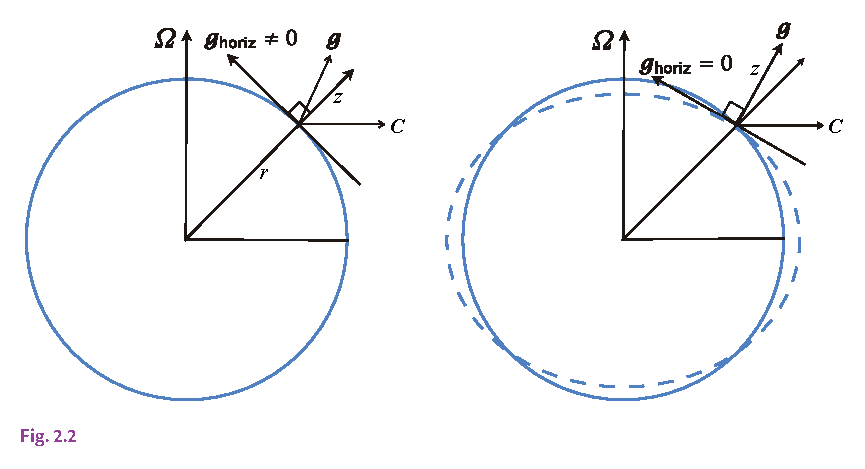
\includegraphics[width=\textwidth]{assets/fig_centrifugal_force.pdf}
  \caption{
    Left: directions of forces and coordinates in true spherical geometry.
    $\mathbf{g}$ is the effective gravity (including the centrifugal force, $\mathbf{C}$)
    and its horizontal component is evidently non-zero.
    Right: a modified coordinate system, in which the vertical direction is
    defined by the direction of $\mathbf{g}$, and so the horizontal component
    of $\mathbf{g}$ is identically zero. The dashed line schematically indicates
    a surface of constant geopotential.
    The differences between the direction of $\mathbf{g}$ and the direction of
    the radial coordinate, and between the sphere and the geopotential surface,
    are much exaggerated and in reality are similar to the thickness of the
    lines themselves.
    This is Fig. 2.2 in AOFD (Vallis, 2017).
  }
  \label{fig:centrifugal_force}
\end{figure}

\subsection{Coriolis force components}

\begin{figure}[h]
  \centering
  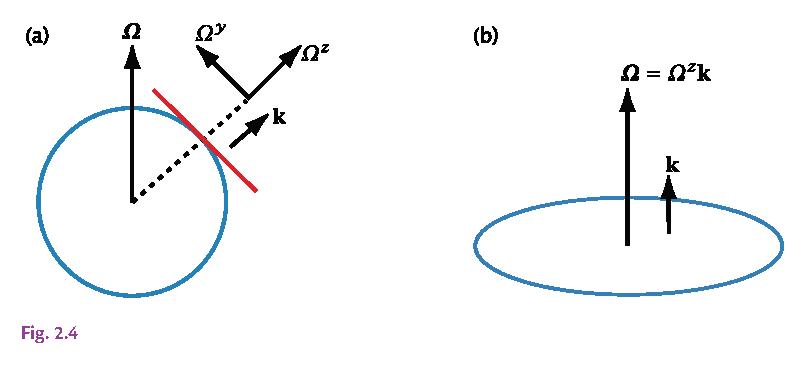
\includegraphics[width=\textwidth]{assets/fig_rotation_components.pdf}
  \caption{
    (a) On the sphere the rotation vector $\mathbf{\Omega}$ can be decomposed
    into two components, one in the local vertical and one in the local horizontal,
    pointing toward the pole. That is, $\mathbf{\Omega} = \Omega_y \mathbf{j} + \Omega_z \mathbf{k}$
    where $\Omega_y = \Omega \cos\theta$ and $\Omega_z = \Omega \sin\theta$.
    In geophysical fluid dynamics, the rotation vector in the local vertical
    is often the more important component in the horizontal momentum equations.
    On a rotating disk, (b), the rotation vector $\mathbf{\Omega}$ is parallel
    to the local vertical $\mathbf{k}$.
    This is Fig. 2.4 in AOFD (Vallis, 2017).
  }
  \label{fig:rotation_components}
\end{figure}

Let's now examine in more detail the effects the Coriolis force on the flow.
The angular velocity $\mathbf{\Omega}$ is a vector that points in the direction
oriented from the center of the Earth toward the North Pole
(see Fig. \ref{fig:rotation_components}).
On the surface of the planet, thus, it has two components: A locally vertical
one, $\Omega_z$, and a meridional one, $\Omega_y$:

\begin{equation}
  \mathbf{\Omega} =
  \begin{bmatrix}
    0 \\
    \Omega_y \\
    \Omega_z
  \end{bmatrix} = 
  \begin{bmatrix}
    0 \\
    \Omega \cos\theta \\
    \Omega \sin\theta
  \end{bmatrix}
\end{equation}
where $\theta$ is the latitude.

The Coriolis force is then:

\begin{equation}
  - 2 \mathbf{\Omega} \times \mathbf{u} =
  \begin{bmatrix}
    \mathbf{i} & \mathbf{j} & \mathbf{k} \\
    0 & - 2 \Omega \cos\theta & - 2 \Omega \sin\theta \\
    u & v & w
  \end{bmatrix} =
  \begin{bmatrix}
    - 2 \Omega w \cos\theta + 2 \Omega v \sin\theta \\
    - 2 \Omega u \sin\theta \\
    2 \Omega u \cos\theta
  \end{bmatrix}
\end{equation}
The Coriolis term thus contributes to all three components of the flow, and
their components vary with latitude.
Let's look at the horizontal components first.
On geophysical scales, generally $w \ll u$ and so the $2 \Omega w \cos\theta$
can often be neglected.
The two dominant horizontal components of the Coriolis force then become
$(-2\Omega v \sin\theta, 2\Omega u \sin\theta)$.
These components are zero at the Equator and increase poleward.
The vertical component, $-2 \Omega u \cos\theta$, can be neglected as well as
its magnitude is very small compared to the other terms in the momentum
equation.

The practical implications of the Coriolis flow is that it deflects it
toward the right on the Northern hemisphere and to the left on the Southern
hemisphere.
Let's now incorporate the Coriolis force components into the vector-component
form of the momentum equation and apply some convenient approximations, namely
the f-plane and the $\beta$-plane approximations.

\subsection{f-plane and $\beta$-plane approximations}

Although geophysical fluids flow on a sphere, the curvature of the surface of
the planet is negligible for many applications.
Here we will make the so-called f-plane approximation in which the flow is
assumed to be on a flat plane tangent to the surface of a curved planet.
The main assumption of the f-plane approximation is that the planet's rotation
exhibits only a locally vertical component anywhere on that planet's surface.
In other words, we'll neglect the horizontal component (\textit{i.e.} $\Omega_y$).
With that assumption, the Coriolis force becomes strictly horizontal:

\begin{equation}
  - 2 \mathbf{\Omega} \times \mathbf{u} =
  \begin{bmatrix}
    2 \Omega v \sin\theta \\
    - 2 \Omega u \sin\theta \\
    0
  \end{bmatrix}
\end{equation}

Let's now define the so-called \textit{Coriolis parameter}\index{Coriolis!parameter}
$f_0 = 2 \Omega_z = 2 \Omega \sin\theta$, so we can write the Coriolis force
more concisely as:

\begin{equation}
  - f_0 \mathbf{k} \times \mathbf{u} =
  \begin{bmatrix}
    f_0 v \\
    - f_0 u \\
    0
  \end{bmatrix}
\end{equation}
The effect of the Coriolis force on the flow is now even more apparent:
A positive meridional flow causes a positive zonal acceleration,
and a positive zonal flow causes a negative meridional acceleration.
The implication of this is that the Coriolis force induces clockwise and
counterclockwise rotations in the Northern and Southern hemispheres,
respectively.

Ignoring viscosity for brevity, we can re-write our system of momentum equations as:

\begin{equation}
  \frac{du}{dt} = - \frac{1}{\rho} \frac{\partial p}{\partial x} + f_0 v
\end{equation}

\begin{equation}
  \frac{dv}{dt} = - \frac{1}{\rho} \frac{\partial p}{\partial y} - f_0 u
\end{equation}

\begin{equation}
  \frac{dw}{dt} = - \frac{1}{\rho} \frac{\partial p}{\partial x} - g
\end{equation}

While on the small plane tangential to the planet's surface the local rotation
may be uniform in space, in reality it does vary with latitude:

\begin{equation}
  f = 2 \Omega \sin\theta \approx 2\Omega \sin\theta_0 + 2\Omega (\theta - \theta_0) \cos\theta_0
\end{equation}
from small deviations in $\theta$.
On a plane, the above can be expressed as:

\begin{equation}
f = f_0 + \beta y
\end{equation}
where $f_0 = 2\Omega \sin\theta_0$ and $\beta = \partial f/\partial y = (2\Omega\cos\theta_0) / R_E$
(where $R_E$ is the radius of the Earth).

\subsection{Geostrophic balance}

Now that we have incorporated the effects of rotation into our equations of motion,
let's evaluate the scales of the terms in the horizontal momentum equations.
We will start from Eq. \ref{eq:momentum_navier_stokes_rotating}, use the f-plane
notation for the Coriolis term, ignore the viscous terms, and drop the gravity
term as we're looking at the flow in the horizontal plane:

\begin{equation}
  \frac{\partial \mathbf{u}}{\partial t} +
  (\mathbf{u} \cdot \nabla) \mathbf{u} +
  \mathbf{f} \times \mathbf{u} =
  - \frac{1}{\rho} \nabla p
\end{equation}

As we did in Section \ref{sec:nondimensionalization_and_scaling}, let's scale
each term on the left-hand side with their characteristic scales for mesoscale
ocean flow ($L \sim 10^5\ m$, $T \sim 10^6\ s$, $U \sim 10^{-1}\ m/s$):

\begin{itemize}
  \item $\frac{\partial \mathbf{u}}{\partial t} \sim \frac{U}{T} \sim 10^{-7}$
  \item $(\mathbf{u} \cdot \nabla) \mathbf{u} \sim \frac{U^2}{L} \sim 10^{-7}$
  \item $\mathbf{f} \times \mathbf{u} \sim f_0 U \sim 10^{-6}$
\end{itemize}
This means that on these oceanic scales ($L \sim 100\ km$, $T \sim 1\ day$),
the inertial terms are of the same order of magnitude as the Coriolis term.
In other words, rotation here is much more important than the local rate of
change or advection.
Also, whatever the scale of the pressure gradient term is, it is the only
term that can balance the rotation.
Thus, if we can state that the inertial terms can be neglected, we can also
state:

\begin{equation}
  \mathbf{f} \times \mathbf{u} \approx - \frac{1}{\rho} \nabla p
\end{equation}
or, in scalar component form:

\begin{equation}
  f u \approx - \frac{1}{\rho} \frac{\partial p}{\partial y}
\end{equation}

\begin{equation}
  f v \approx \frac{1}{\rho} \frac{\partial p}{\partial x}
\end{equation}

This balance is called the
\textit{geostrophic balance}\index{Geostrophic!balance}\index{Balance!geostrophic},
and it is a key concept in geophysical fluid dynamics.
It states that the flow is governed by the balance between the rotation and the
pressure gradient force.
Although the geostrophic balance is strictly an approximation and it never holds
exactly, large scale oceanic ($L \sim 100\ km$ and larger) and atmospheric
($L \sim 1000\ km$ and larger) flows are often in geostrophic balance.
For the analysis of geophysical flows at such scales, it is then useful to
define the \textit{geostrophic velocity}\index{Geostrophic!velocity} as:

\begin{equation}
  u_g = - \frac{1}{\rho f} \frac{\partial p}{\partial y}
\end{equation}

\begin{equation}
  v_g = \frac{1}{\rho f} \frac{\partial p}{\partial x}
\end{equation}
Notice that the geostrophic flow is always perpendicular to the pressure gradient,
which means it is parallel to the isobars (lines of constant pressure).
This also means that the isobars are streamlines of the geostrophic flow.
In the northern hemisphere ($f > 0$), the geostrophic flow is cyclonic
(counter-clockwise) around the low-pressure region and anti-cyclonic
(clockwise) around the high-pressure region.
In the southern hemisphere ($f < 0$), it is the opposite.
A nearly geostrophic flow is illustrated in Fig. \ref{fig:geostrophic_flow}.

\begin{figure}[h]
  \centering
  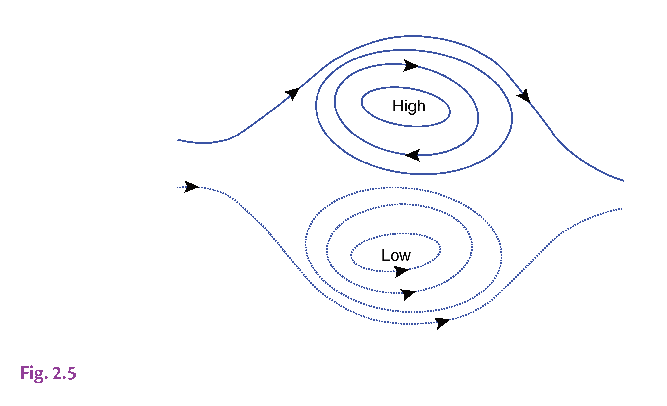
\includegraphics[width=0.8\textwidth]{assets/fig_geostrophic_balance.pdf}
  \caption{
    Geostrophic flow with a positive value of the Coriolis parameter $f$.
    Flow is parallel to the lines of constant pressure (isobars).
    Cyclonic flow is anticlockwise around a low pressure region and
    anticyclonic flow is clockwise around a high. If $f$ were negative, as in
    the Southern Hemisphere, (anti)cyclonic flow would be (anti)clockwise.
    This is Fig. 2.5 in AOFD (Vallis, 2017).
  }
  \label{fig:geostrophic_flow}
\end{figure}

\subsection{Rossby number}

Recall that we required the inertial terms to be much smaller than the Coriolis
term for the geostrophic approximation to hold.
Like we did earlier with the Reynolds number to quantify how turbulent a flow is,
we can define the \textit{Rossby number}\index{Rossby!number} as:

\begin{equation}
  \text{Ro} \equiv
  \frac{\text{Advection}}{\text{Rotation}} = 
  \frac{\left( \mathbf{u} \cdot \nabla \right) \mathbf{u}}{\mathbf{f} \times \mathbf{u}}
  \approx \frac{\frac{U^2}{L}}{fU}
  \approx \frac{U}{fL}
\end{equation}
Though the Rossby number characterizes the relative importance of rotation in
the flow, notice that the rotation term is in the denominator.
The Rossby number is thus small for flows in which rotation dominates over
advection.
In general, flows with a Rossby number of 0.1 or smaller are considered
approximately geostrophically balanced.

\subsection{Exercises}

\begin{enumerate}
  \item Calculate the effective gravity at the Earth's Equator, poles, and 45 degrees
  latitude, taking into effect centrifugal acceleration.
  \item Using scale analysis, show that on geophysical scales the vertical
  component of the Coriolis force is negligible compared to the other terms
  in the momentum equation.
  \item Derive the Coriolis parameter $f$ on the $\beta$-plane assuming small
  variation in latitude $\theta$ around the constant $\theta_0$ at which $f = f_0$.
\end{enumerate}

\subsection*{Further reading}

\begin{itemize}
  \item Sections 2.1-2.3 of \textit{EAOD} by Vallis
\end{itemize}

\newpage
\section{Stratified flows}

We derived our equations for mass and momentum conservation and we incorporated
the effects of rotation.
We also explored how the density may vary in the vertical according to the
ideas gas law (in the atmosphere) or the equation of state for seawater.
We now explore the effects of stratification on the flow and examine the
common approximations used for large-scale oceanic flows.

\subsection{The Boussinesq equations}

The \textit{Boussinesq approximation}\index{Boussinesq!approximation} is an
approximation to the full equations of motion.
It assumes that the density and pressure perturbations are much smaller than
their means, and when applied to the Navier-Stokes equations, results in the
\textit{Boussinesq equations}\index{Boussinesq!equations}.

We start by decomposing the density and pressure into the mean and the
perturbation components:

\begin{equation}
  \rho = \rho_0 + \delta \rho(x, y, z, t)
  \label{eq:boussinesq_density}
\end{equation}

\begin{equation}
  p = p_0 + \delta p(x, y, z, t)
  \label{eq:boussinesq_pressure}
\end{equation}
where $\rho_0$ and $p_0$ are the mean density and pressure, respectively,
and $\delta \rho$ and $\delta p$ are their respective perturbations.
For both quantities, we will require that their perturbations are much smaller
than the means, \textit{i.e.} $\delta \rho \ll \rho_0$, $\delta p \ll p_0$.
Since $\rho_0$ and $p_0$ are constant, the hydrostatic approximation is
trivially satisfied:

\begin{equation}
  \frac{d p_0}{d z} = - \rho_0 g
\end{equation}

\subsection{Momentum balance}

Let's first apply the Boussinesq approximation to the momentum balance.
Recall the Navier-Stokes equation with rotation
(Eq. \ref{eq:momentum_navier_stokes_rotating}), while neglecting the viscosity
term:

\begin{equation}
  \frac{d \mathbf{u}}{dt} = - \frac{1}{\rho} \nabla p - f \mathbf{k} \times \mathbf{u} + \mathbf{g}
\end{equation}
Apply Eqs. \ref{eq:boussinesq_density}-\ref{eq:boussinesq_pressure} to the
above equation to get:

\begin{equation}
  \left( \rho_0 + \delta \rho \right) \left( \frac{d \mathbf{u}}{dt} + \mathbf{f} \times \mathbf{u} \right) =
  - \nabla \left( p_0 + \delta p \right)
  + \left( \rho_0 + \delta \rho \right) \mathbf{g}
\end{equation}

\begin{equation}
  - \nabla \left( p_0 + \delta p \right) =
  - \nabla \delta p - \frac{\partial p_0}{\partial z} \mathbf{k} = 
  - \nabla \delta p - \rho_0 \mathbf{g}
\end{equation}
Now, recall that $\delta \rho \ll \rho_0$, so we can drop the $\delta \rho$
on the left-hand side:

\begin{equation}
  \rho_0 \left( \frac{d \mathbf{u}}{dt} + \mathbf{f} \times \mathbf{u} \right) =
  - \nabla \delta p + \delta \rho\ \mathbf{g}
\end{equation}

\begin{equation}
  \frac{d \mathbf{u}}{dt} + \mathbf{f} \times \mathbf{u} =
  - \frac{1}{\rho_0} \nabla \delta p + \frac{\delta \rho}{\rho_0} \mathbf{g}
\end{equation}
For convenience of notation, let's now define \textit{buoyancy}\index{buoyancy}
as $b = - g \delta \rho / \rho_0$, and re-write the above to obtain the
Boussinesq momentum equation:

\begin{equation}
  \frac{d \mathbf{u}}{dt} + \mathbf{f} \times \mathbf{u} =
  - \frac{1}{\rho_0} \nabla \delta p + b \mathbf{k}
\end{equation}
This equation states that now that we are in a gradually stratified fluid,
the gravity term is scaled by $\delta \rho / \rho_0$ to yield the appropriate
vertical acceleration, and the pressure gradient is due to the relatively
small perturbations in density $\delta \rho$ around  the mean density $\rho_0$.

\subsection{Continuity}

As we did for the momentum equation, we'll now apply the Boussinesq approximation
(\textit{i.e.} $\rho = \rho_0 + \delta \rho$, $\delta \rho \ll \rho_0$) to the
continuity equation.
Recall the continuity equation in its complete form:

\begin{equation}
  \frac{d \rho}{dt} + \rho \nabla \cdot \mathbf{u} = 0
\end{equation}
Insert Eq. \ref{eq:boussinesq_density} to get:

\begin{equation}
  \frac{d\delta \rho}{dt} + \left( \rho_0 + \delta \rho \right) \nabla \cdot \mathbf{u} = 0
\end{equation}
Then, if we can state that that $d\delta \rho / dt \ll \rho_0 \nabla \cdot \mathbf{u}$,
which we will for the Boussinesq approximation, we recover the original
continuity equation for incompressible flows:

\begin{equation}
  \nabla \cdot \mathbf{u} = 0
\end{equation}
Note that we do not say that strictly $d \delta \rho / dt = 0$, but rather that
we can neglect it in this equation in favor of the velocity divergence term.
The evolution of $\delta \rho$ is still governed by the evolution of buoyancy,
which in turn is governed by the evolution of the temperature and salinity fields
and the equation of state.
The buoyancy $b = - g \delta \rho / \rho_0$ evolves as:

\begin{equation}
  \frac{d b}{dt} = \dot{b}
\end{equation}
and the equation of state can be expressed in terms of buoyancy:

\begin{equation}
  b = b(T, S, p)
\end{equation}
which is just another form of Eq. \ref{eq:equation_of_state_ocean}.

Finally the temperature and salinity evolve as before, following
Eqs. \ref{eq:temperature_equation_ocean} and \ref{eq:salinity_equation_ocean},
respectively.

\subsection{Complete system of equations}

The full system of Boussinesq equations for the ocean are then:

\begin{equation}
  \frac{d \mathbf{u}}{dt} + \mathbf{f} \times \mathbf{u} =
  - \frac{1}{\rho_0} \nabla \delta p + b \mathbf{k}
\end{equation}

\begin{equation}
  \nabla \cdot \mathbf{u} = 0
\end{equation}

\begin{equation}
  \frac{d T}{dt} = \dot{T}
\end{equation}

\begin{equation}
  \frac{d S}{dt} = \dot{S}
\end{equation}

\begin{equation}
  b = b(T, S, p)
\end{equation}


%\newpage
%\section{Boundary layers}

%\newpage
%\section{Turbulence}

%\newpage
%\section{Surface gravity waves}

\newpage
\appendix

\section{Quick reference}

This section serves a quick reference for the key equations used in this book.\\

\textbf{Gradient:}

\begin{equation}
  \nabla = \frac{\partial}{\partial x} \mathbf{i} + \frac{\partial}{\partial y} \mathbf{j} + \frac{\partial}{\partial z} \mathbf{k}
\end{equation}

\textbf{Divergence:}

\begin{equation}
  \nabla \cdot \mathbf{u} = \frac{\partial u}{\partial x} + \frac{\partial v}{\partial y} + \frac{\partial w}{\partial z}
\end{equation}

\textbf{Curl:}

\begin{equation}
  \nabla \times \mathbf{u} = \left( \frac{\partial w}{\partial y} - \frac{\partial v}{\partial z} \right) \mathbf{i} + \left( \frac{\partial u}{\partial z} - \frac{\partial w}{\partial x} \right) \mathbf{j} + \left( \frac{\partial v}{\partial x} - \frac{\partial u}{\partial y} \right) \mathbf{k}
\end{equation}

\textbf{Laplacian:}

\begin{equation}
  \nabla^2 = \frac{\partial^2}{\partial x^2} + \frac{\partial^2}{\partial y^2} + \frac{\partial^2}{\partial z^2}
\end{equation}

\textbf{Lagrangian derivative operator:}
 
\begin{equation}
  \frac{d}{dt} = \frac{\partial}{\partial t} + (\mathbf{u} \cdot \nabla)
\end{equation}

\textbf{Continuity, Eulerian form:}

\begin{equation}
  \frac{\partial \rho}{\partial t} + \nabla (\rho \mathbf{u}) = 0
\end{equation}

\textbf{Continuity, Lagrangian form:}

\begin{equation}
  \frac{d\rho}{dt} + \rho \nabla \cdot \mathbf{u} = 0
\end{equation}

\textbf{Momentum, Cauchy:}

\begin{equation}
  \frac{\partial \mathbf{u}}{\partial t} + (\mathbf{u} \cdot \nabla) \mathbf{u} =
  \frac{1}{\rho} \nabla \cdot \boldsymbol{\sigma} + \frac{\mathbf{F}_b}{\rho}
\end{equation}

\textbf{Stress tensor as a combination of pressure and deviatoric stress:}

\begin{equation}
  \boldsymbol{\sigma} = -p \mathbf{I} + \boldsymbol{\tau}
\end{equation}

\textbf{Momentum, Euler:}

\begin{equation}
  \frac{\partial \mathbf{u}}{\partial t} + (\mathbf{u} \cdot \nabla) \mathbf{u} =
  - \frac{1}{\rho} \nabla p
\end{equation}

\textbf{Momentum, Navier-Stokes:}

\begin{equation}
  \frac{\partial \mathbf{u}}{\partial t} + (\mathbf{u} \cdot \nabla) \mathbf{u} =
  - \frac{1}{\rho} \nabla p + \nu \nabla^2 \mathbf{u} + \frac{\mathbf{F}_b}{\rho}
\end{equation}

\textbf{Momentum, with body force (gravity):}

\begin{equation}
  \frac{\partial \mathbf{u}}{\partial t} + (\mathbf{u} \cdot \nabla) \mathbf{u} =
  - \frac{1}{\rho} \nabla p + \mathbf{g} + \nu \nabla^2 \mathbf{u}
\end{equation}

\textbf{Momentum, Navier-Stokes, in scalar form:}

\begin{equation}
  \frac{\partial u}{\partial t} + 
  u \frac{\partial u}{\partial x} + 
  v \frac{\partial u}{\partial y} + 
  w \frac{\partial u}{\partial z} = 
  - \frac{1}{\rho} \frac{\partial p}{\partial x} + \nu \left( \frac{\partial^2 u}{\partial x^2} + \frac{\partial^2 u}{\partial y^2} + \frac{\partial^2 u}{\partial z^2} \right)
\end{equation}

\begin{equation}
  \frac{\partial v}{\partial t} + 
  u \frac{\partial v}{\partial x} + 
  v \frac{\partial v}{\partial y} + 
  w \frac{\partial v}{\partial z} = 
  - \frac{1}{\rho} \frac{\partial p}{\partial y} + \nu \left( \frac{\partial^2 v}{\partial x^2} + \frac{\partial^2 v}{\partial y^2} + \frac{\partial^2 v}{\partial z^2} \right)
\end{equation}

\begin{equation}
  \frac{\partial w}{\partial t} + 
  u \frac{\partial w}{\partial x} + 
  v \frac{\partial w}{\partial y} + 
  w \frac{\partial w}{\partial z} = 
  - \frac{1}{\rho} \frac{\partial p}{\partial z} - g + \nu \left( \frac{\partial^2 w}{\partial x^2} + \frac{\partial^2 w}{\partial y^2} + \frac{\partial^2 w}{\partial z^2} \right)
\end{equation}

\textbf{Equation of state, moist air:}

\begin{equation}
  p = \rho R_d T \left[1 + q \left(\frac{R_v}{R_d} - 1 \right) \right]
\end{equation}

\textbf{Equation of state, seawater:}

\begin{equation}
  \rho = \rho_0 \left[ 1 - \beta_T(T-T_0) + \beta_S(S-S_0) - \beta_p(p-p_0) \right]
\end{equation}

\textbf{Hydrostatic approximation:}

\begin{equation}
  \frac{dw}{dt} = 0
\end{equation}

\begin{equation}
  \frac{\partial p}{\partial z} = -\rho g
\end{equation}

\textbf{Rate of change of a rotating vector:}

\begin{equation}
  \left(\frac{d\mathbf{C}}{dt}\right)_I = \mathbf{\Omega} \times \mathbf{C}
\end{equation}

\textbf{Rate of change of a rotating vector in a rotating frame:}

\begin{equation}
  \left(\frac{d\mathbf{B}}{dt}\right)_I = \left(\frac{d\mathbf{B}}{dt}\right)_R + \mathbf{\Omega} \times \mathbf{B}
\end{equation}

\textbf{Rate of change of velocity in a rotating frame:}

\begin{equation}
  \left( \frac{d \mathbf{u}_R}{dt} \right)_R =
  \left( \frac{d \mathbf{u}_I}{dt} \right)_I -
  2 \mathbf{\Omega} \times \mathbf{u}_R -
  \mathbf{\Omega} \times \left( \mathbf{\Omega} \times \mathbf{r} \right)
\end{equation}

\textbf{Navier-Stokes equation with rotation:}

\begin{equation}
  \frac{\partial \mathbf{u}}{\partial t} +
  \left( \mathbf{u} \cdot \nabla \right) \mathbf{u} =
  - \frac{1}{\rho} \nabla p
  - \frac{1}{\rho} \nabla \Phi
  - 2 \mathbf{\Omega} \times \mathbf{u}
  + \nu \nabla^2 \mathbf{u}
\end{equation}

\textbf{Coriolis parameter:}

\begin{equation}
  f = 2 \Omega \sin(\theta)
\end{equation}

\textbf{$f$-plane approximation:}

\begin{equation}
  f = f_0 = 2 \Omega \sin(\theta_0)
\end{equation}

\textbf{$\beta$-plane approximation:}

\begin{equation}
  f = f_0 + \beta y
\end{equation}

\begin{equation}
  \beta = \frac{\partial f}{\partial y} = \frac{2\Omega\cos(\theta_0)}{R_E}
\end{equation}

\textbf{Geostrophic balance:}

\begin{equation}
  \mathbf{f} \times \mathbf{u} = - \frac{1}{\rho} \nabla p
\end{equation}

\textbf{Geostrophic velocity:}

\begin{equation}
  u_g = - \frac{1}{\rho f} \frac{\partial p}{\partial y}
\end{equation}

\begin{equation}
  v_g = \frac{1}{\rho f} \frac{\partial p}{\partial x}
\end{equation}

\textbf{Rossby number:}

\begin{equation}
  \text{Ro} \equiv \frac{\left( \mathbf{u} \cdot \nabla \right) \mathbf{u}}{\mathbf{f} \times \mathbf{u}} \approx \frac{U}{fL}
\end{equation}

\printindex

\end{document}
